\chapter{Mass fits}
\label{sec:rkst_fits}

In order to extract the yields of the rare and normalisation channels unbinned maximum likelihood fits
to the 4-body invariant masses $m(K\pi\ell\ell)$ are performed.
The following sections contain a description of the line shapes used to model the signal and background
components in each sample.
These fits are performed simultaneously on the resonant and rare channels.
This method allows to share parameters between the two e.g. those describing data-simulation differences.
The yields of the rare channels are parameterised as a function of the corresponding \jpsi yields as

\begin{equation}
N_{\ell\ell} = N_{\jpsi} \cdot \varepsilon^{ref} \cdot R_{\ell\ell}.
\end{equation}

In this formula $\varepsilon^{ref}$ is the relative efficiency given in Tab.~\ref{tab:RKst_releff} and
$R_{\ell\ell}$ corresponds to the efficiency corrected ratio of the raw rare and resonant yields:

\begin{equation}
R_{\ell\ell} = \frac{\varepsilon^{\jpsi} \cdot N_{\ell\ell}}{\varepsilon^{\ell\ell} \cdot N_{\jpsi}}.
\end{equation}

The two ratios $R_{ee}$ and $R_{\mu\mu}$ are then be used to build
the $R_{\Kstar}$ quantity, as described in Sec.~\ref{sec:RKst_result}.


\section{Mass fits: muonic channels}

For the rare and resonant \mumu channels the fitted variable is the $m(K\pi \mu\mu)$ invariant mass coming
from a kinematic fit where all vertices are required to point to their mother particle.
In the resonant case it is beneficial to also constrain the the dimuon mass to the known \jpsi mass.
The effect of the kinematical fit is to improve the mass resolution by roughly a factor of 2, which results
a more stable fit. Furthermore, misreconstructed events are pushed away from the $\Bz$ peak, which allows to
use a wider mass window to better constrain the combinatorial background slope.
The mass spectrum is fitted in the range $5150 - 5800 ~\mbox{MeV/c}{^2}$ with the lower limit
of the mass range chosen to exclude partially reconstructed background.
As it is not needed to model misreconstructed backgrounds in the fit this also
eliminates systematic uncertainties associated with the knowledge of its shape. 

The PDF chosen to describe the signal in both the $\Bz \to\Kstar\mumu$ and its relative $J/\psi$ channel 
is a Double Crystal Ball function already described in \ref{sec:Lb_fit}.

%A Crystal Ball function
%(Eq. \ref{CB})\cite{Skwarnicki:1986xj} is a probability density function commonly used to model various processes involving energy loss at low energy.
%In particular it is used to model the radiative tail which can be seen in many resonances' peak. This function consists of a Gaussian core and a power-law tail,
%below a certain threshold. The function itself and its first derivative are both continuous.

%\begin{equation}
%C(x;\alpha,n,\bar{x},\sigma) = N \cdot
%\begin{cases}
%exp \left( -\frac{(x - \bar{x})^2}{2\sigma} \right)  & \mbox{   if   } \frac{(x - \bar{x})}{\sigma} > \alpha \\
%A\left( B - \frac{(x - \bar{x})}{\sigma} \right)^{-n} & \mbox{   if   } \frac{(x - \bar{x})}{\sigma} < \alpha
%\end{cases}
%\end{equation}

%where for normalisation and continuity

%\begin{equation}
%\label{CB}
%\begin{array}{ll}
%A = \left( \frac{c}{|\alpha|} \right))^n \cdot exp(- \frac{\alpha^2}{2}) \\
%B = \frac{n}{|\alpha|} - |\alpha|
%\end{array}
%\end{equation}

%A double Crystal Ball is then given by the sum of two Crystal Balls where the parameters of the tail and the mean are kept in common, so that the only free
%parameter added are the $\sigma$ of the second Crystal Ball and the fraction ($f$) of events falling in it.

%\begin{equation}
%\label{DCB}
%D(x;\alpha,n,\bar{x},\sigma_1, \sigma_2, f) = f \cdot C(x;\alpha,n,\bar{x},\sigma_1) + (1 - f) \cdot C(x;\alpha,n,\bar{x},\sigma_2)
%\end{equation}

As a first step simulated distributions are fit using the signal model.
%Independent fits are preformed to the simulated resonant sample and the rare samples in each \qsq bin.
The fitted MC distribution for the resonant channel is reported in Fig.~\ref{fig:mumu_MC_fits}.
%where it is evident that the tail parameters depend on \qsq. This is due mainly to bin migration
%effects that cause the bremsstrahlung tail to be reduced at high \qsq.

For the fit to real data the signal parameters are fixed to the ones found for the simulated samples.
In order to account for possible data-simulation discrepancies a scale factor is multiplied to the widths
and a shift is added to the masses. In summary the PDFs used for the signal fits on data are defined as

\begin{align}
\label{eq:DCB_RKst}
P(x;c,m_0) = & f^{*} \cdot C(x;\alpha_1^{*},n_1^{*},c \cdot \sigma_1^{*}, m^{*} + m_0) \\
&+ (1 - f^{*}) \cdot C(x;\alpha_2^{*},n_2^{*},c \cdot \sigma_2^{*}, m^{*} + m_0)
\end{align}  

where the free parameters are the width scale factor, $c$, and the mass shift, $m_0$, which are common between the rare
and resonant samples. The other parameters, denoted with $*$, are taken from the fit to simulated events, 
separately for the rare and resonant samples and are fixed in the fit on data.
The parameter $f^{*}$ in the formula is the relative fraction of candidates falling in the first Crystal Ball function.

To model the combinatorial background an exponential function was used.
This is the only background component for the rare channel.
In the normalisation channel fit the $\Bs  \to \Kstar\jpsi$ background
is described using the same PDF used for the signal but a different central value, $m$,
which is set at the $\Bs$ nominal mass~\cite{PDG2014}.
Finally, a $\Lb\to\jpsi pK$ background component is modelled using simulated $\Lb\to\jpsi pK$ events
to which the full $\Bz \to \Kstar\jpsi$ selection is applied. The invariant mass distribution
of these candidates is a broad flat shape under the signal peak. The simulated distribution 
is smoothed using a kernel estimation method (using the RooKeysPdf class of the RooFit package~\cite{Verkerke:2003ir}).

In summary the floating variables in the simultaneous fit to rare and resonant \mumu samples are:
the signal and background yields, the combinatorial background slopes, the widths scale $c$ and
the the mass shift $m_0$.

Fig.~\ref{fig:mumu_data_fits} reports fits to real data distributions for the rare and resonant
\mumu channels. Values of fitted parameters are reported on the plots.



\begin{figure}[h!]
\centering 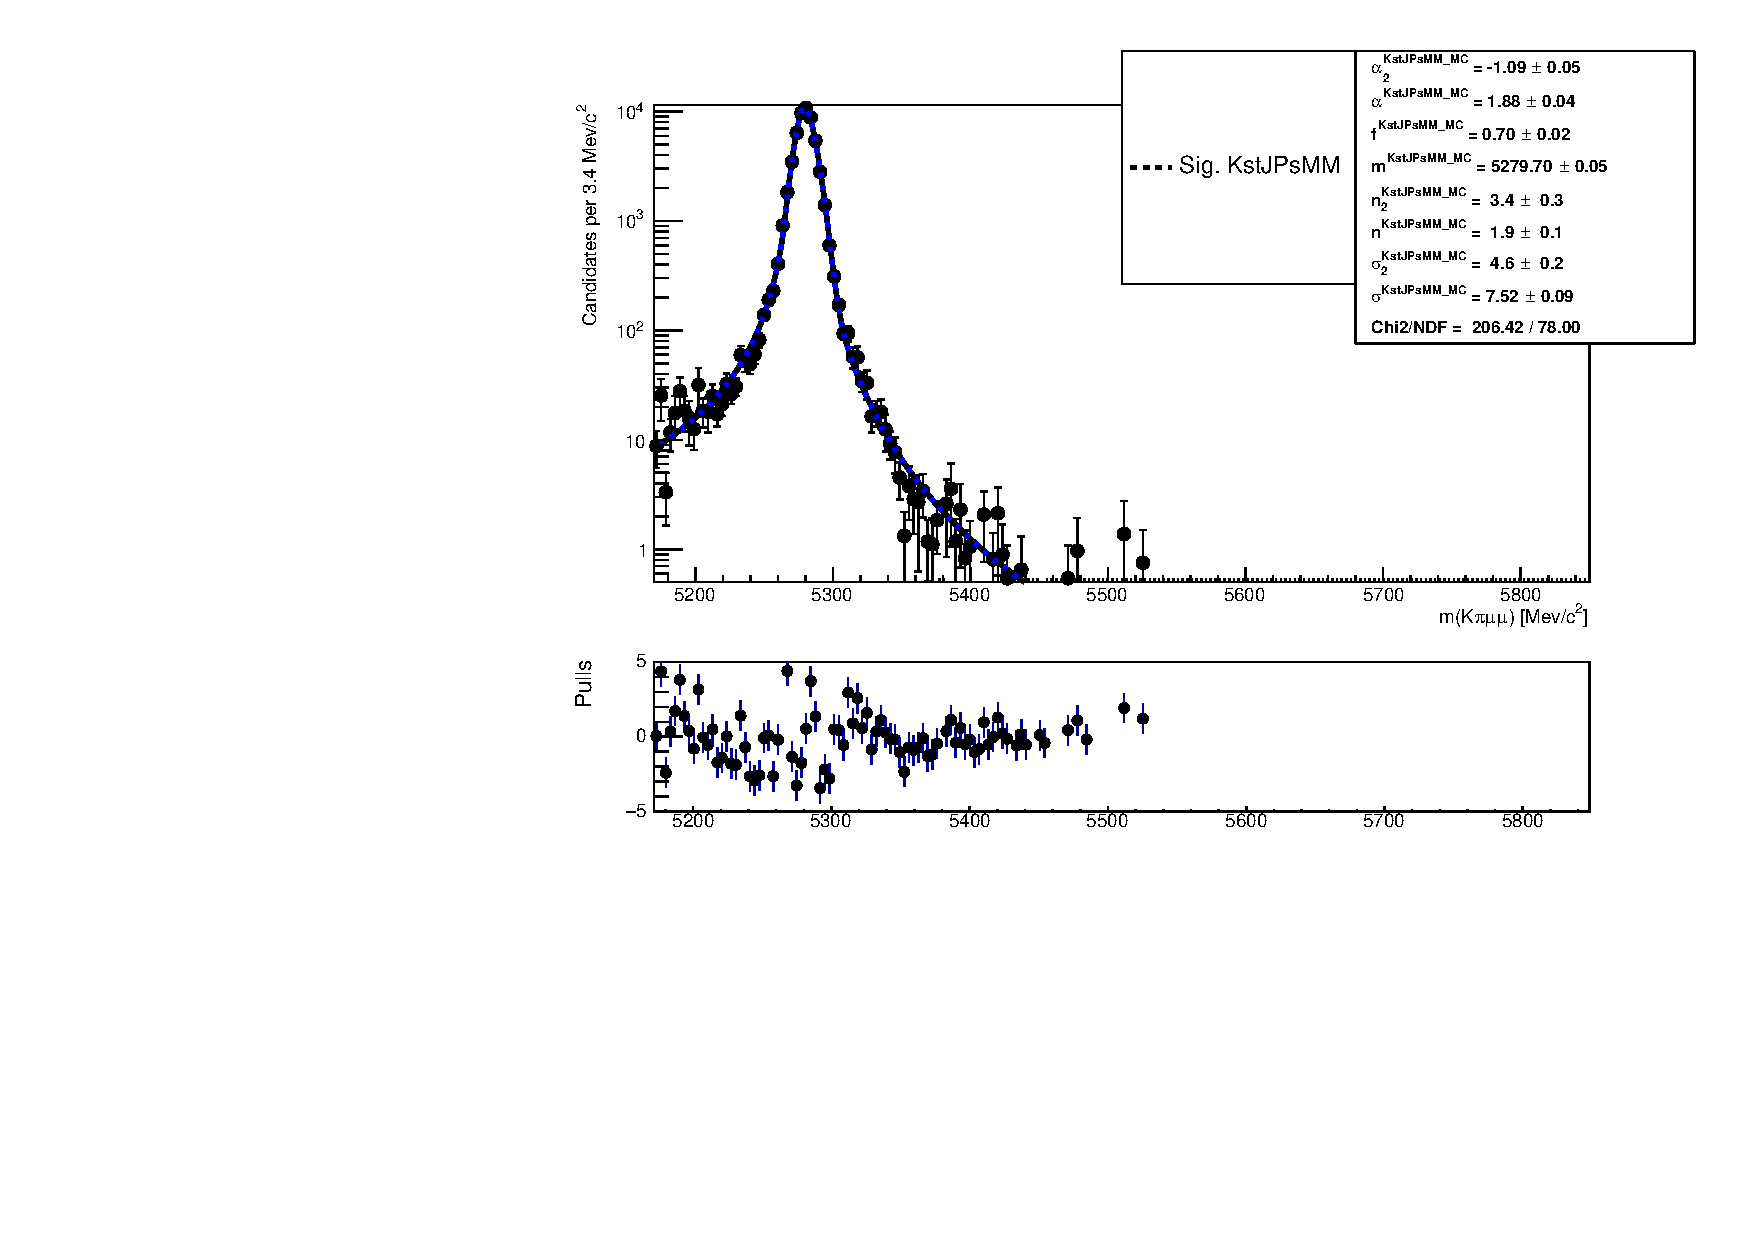
\includegraphics[width=0.8\textwidth]{RKst/figs/fit_MMs_0_MM-q2central-gmc/KstJPsMM_MC_log_fitAndRes.pdf}
%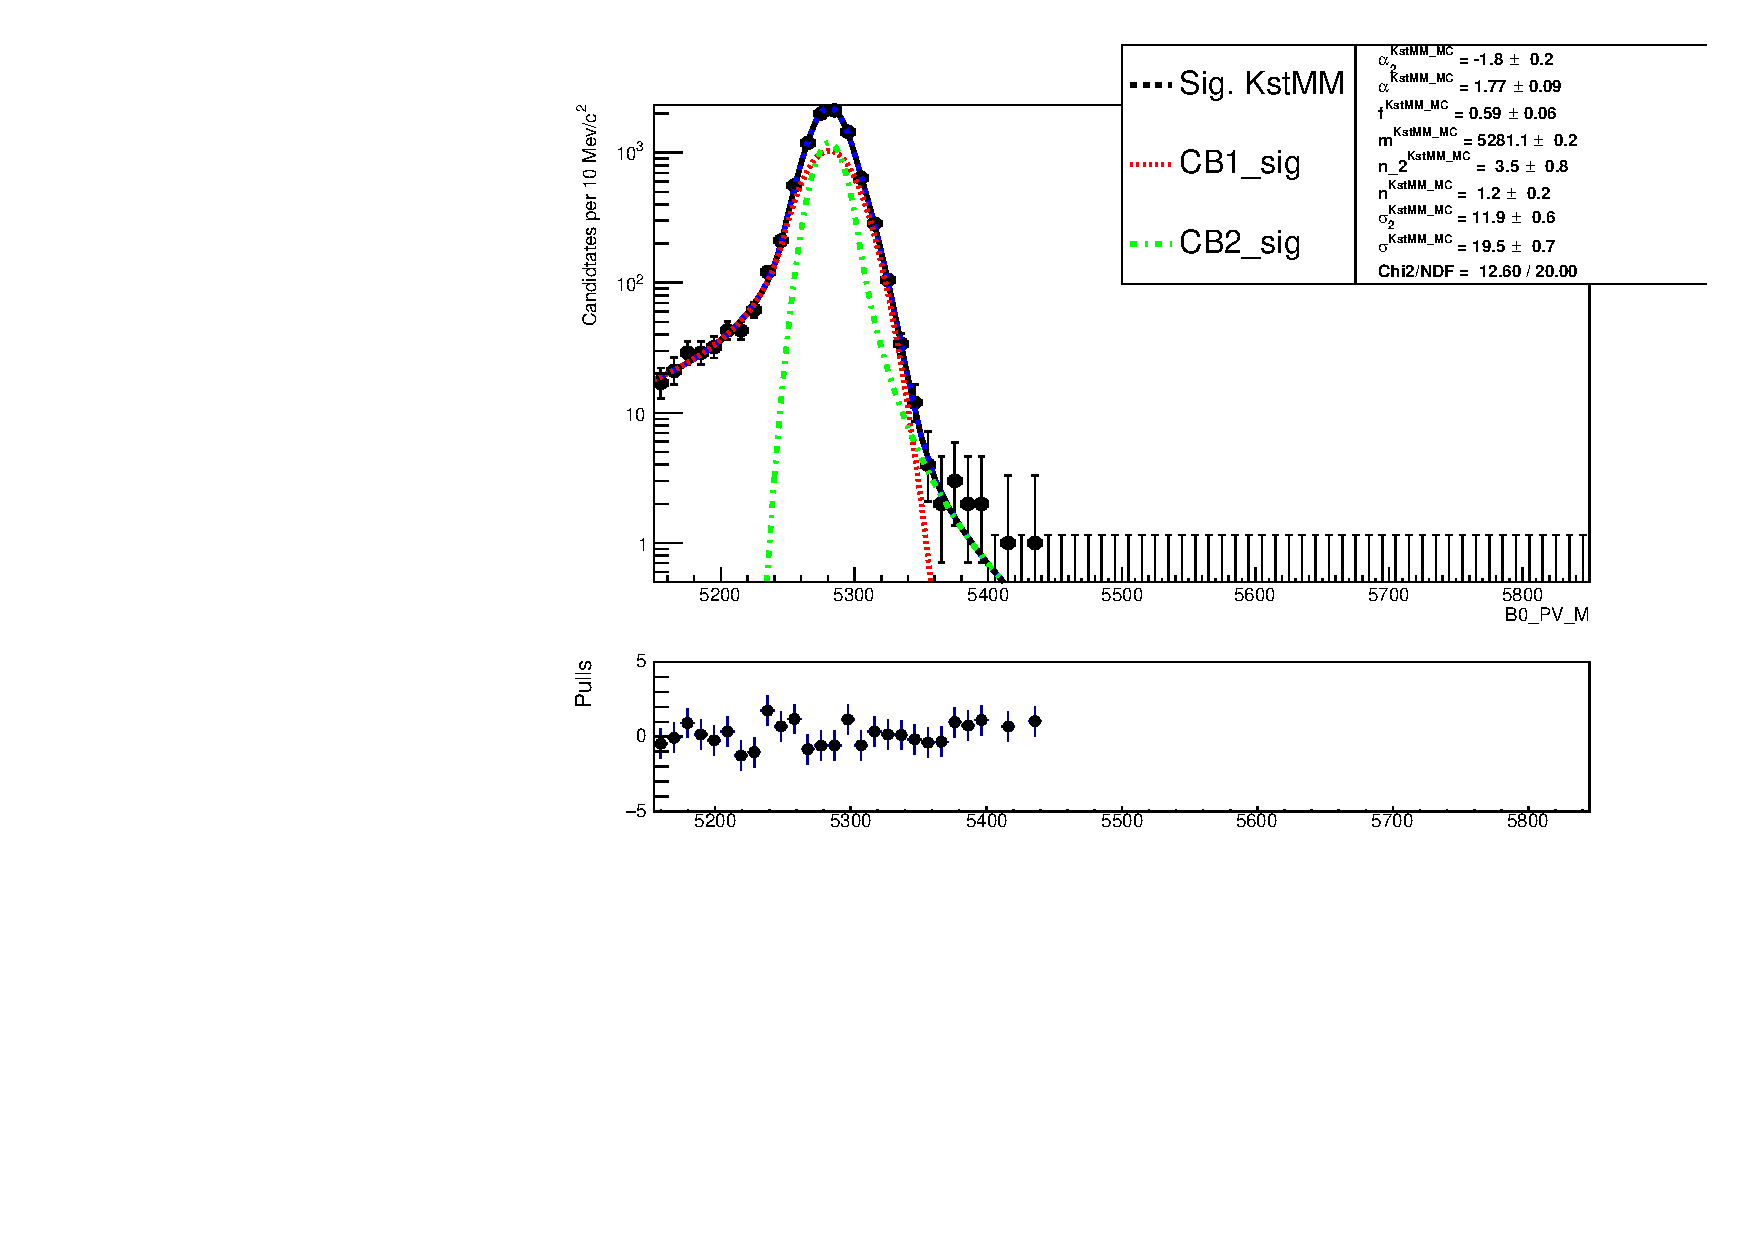
\includegraphics[width=0.48\textwidth]{RKst/figs/Fit/KstMM_MC_log_fitAndRes.pdf}
%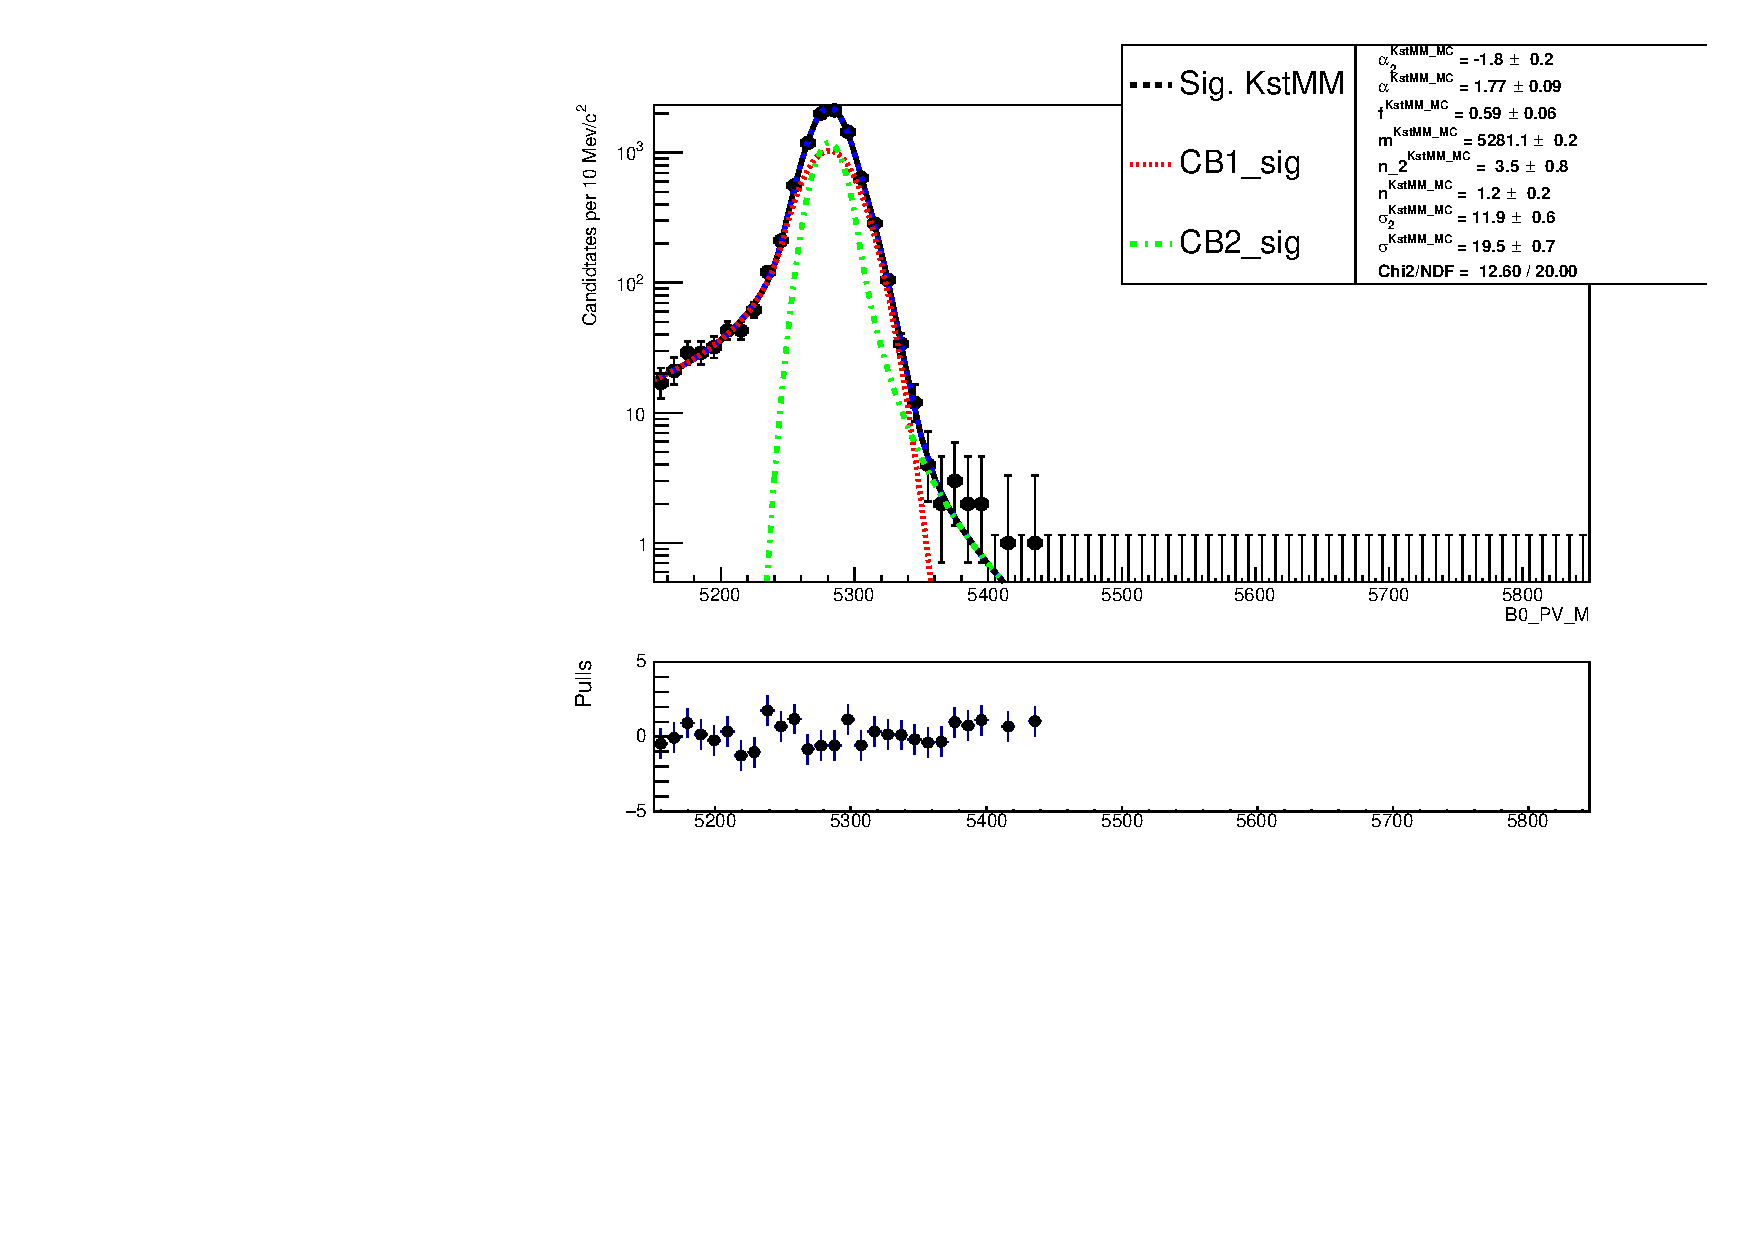
\includegraphics[width=0.48\textwidth]{RKst/figs/Fit/KstMM_MC_log_fitAndRes.pdf}
\caption{Fitted $m(K\pi \mu\mu)$ mass spectrum for $\Kstar\jpsi$ simulated events. }
\label{fig:mumu_MC_fits}
\end{figure}

\begin{figure}[h!]
\centering 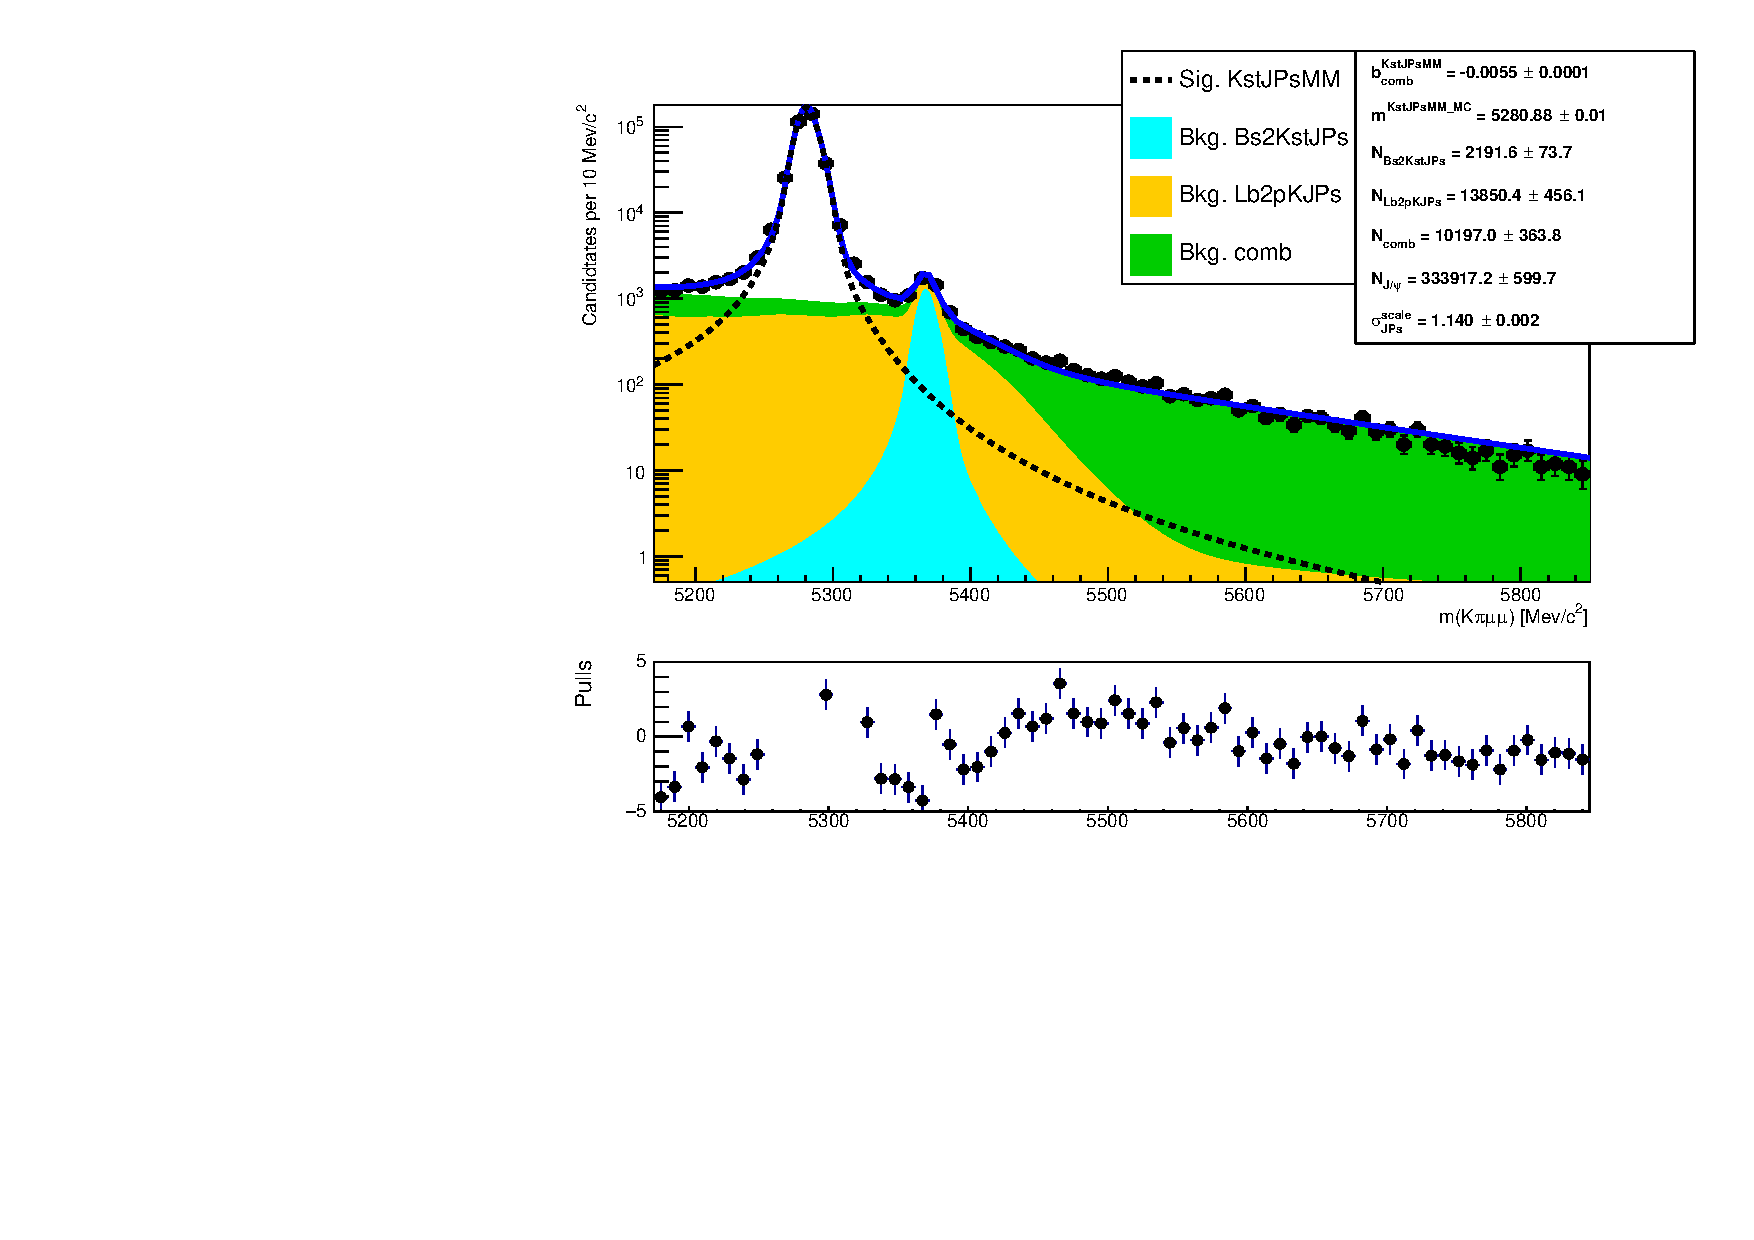
\includegraphics[width=0.8\textwidth]{RKst/figs/fit_MMs_0_MM-q2central-gmc/KstJPsMM_log_fitAndRes.pdf} \\
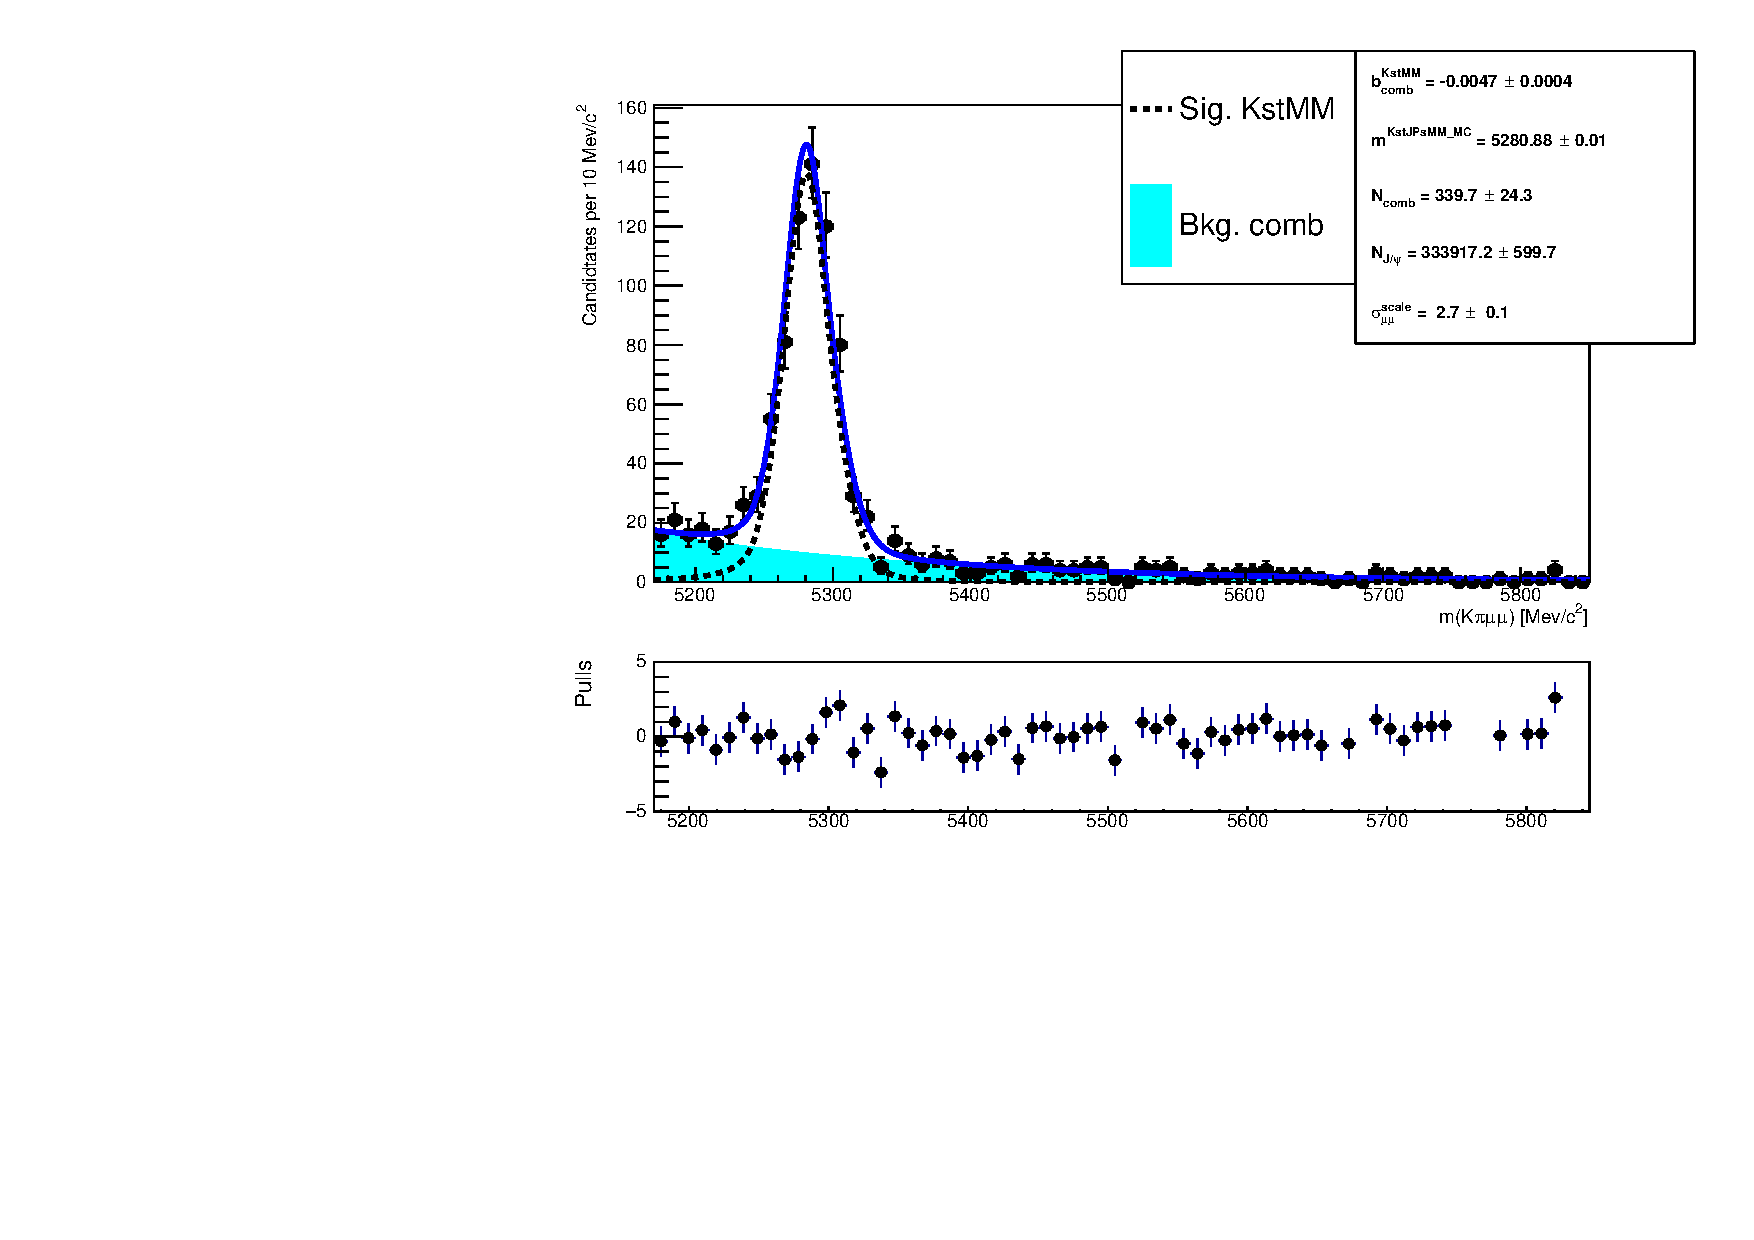
\includegraphics[width=0.48\textwidth]{RKst/figs/fit_MMs_0_MM-q2central-gmc/KstMM_fitAndRes.pdf}
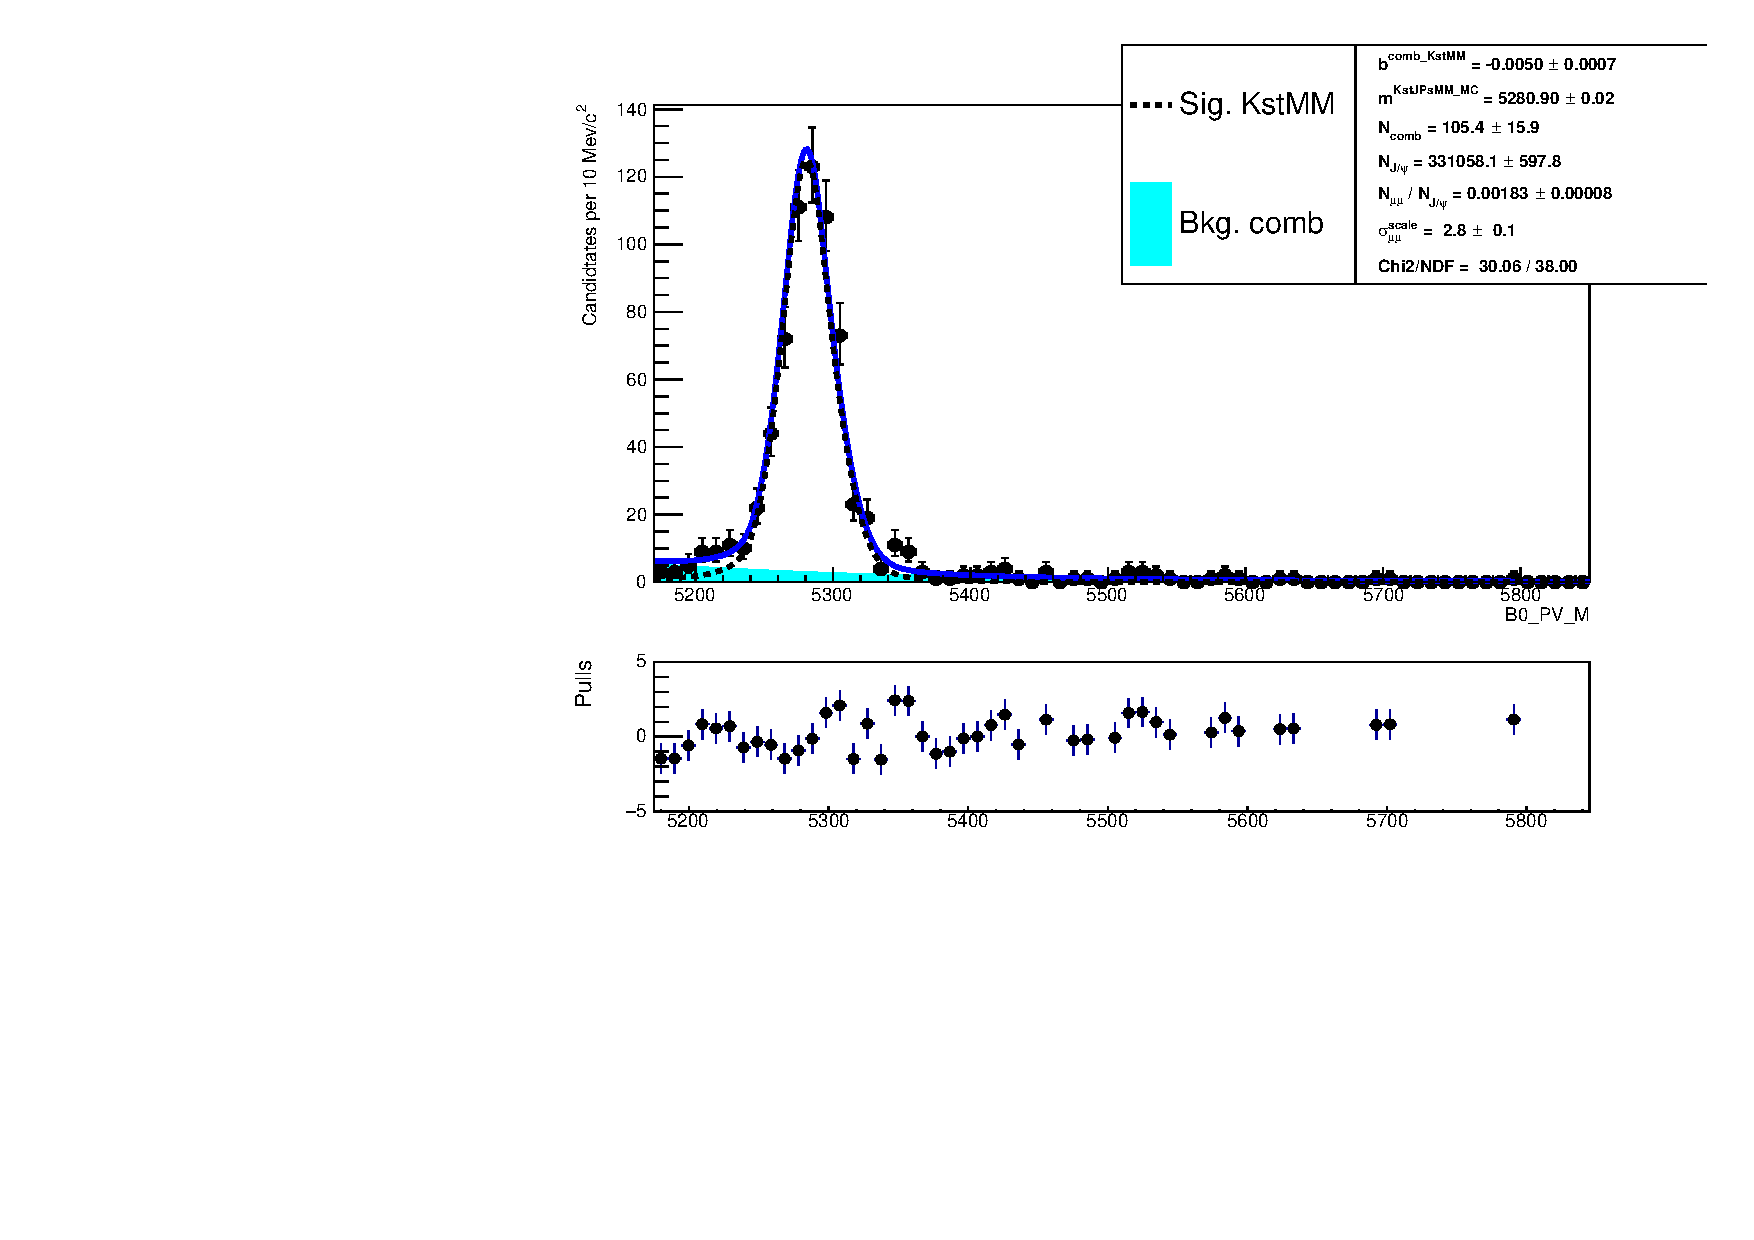
\includegraphics[width=0.48\textwidth]{RKst/figs/fit_MMs_0_MM-q2high-gmc/KstMM_fitAndRes.pdf}
\caption{Fitted $m(K\pi \mu\mu)$ invariant mass spectrum for $\Kstar\jpsi$  (left) and $\Kstar(\jpsi\rightarrow \mumu)$ (right). Dashed lines represent background components. }
\label{fig:mumu_data_fits}
\end{figure}


\section{Mass fits: electronic channels}
\label{sec:RKst_fit_ee}

In the electronic case the variable we fit is the $m(K\pi\ee)$ invariant mass coming from the kinematic
fit where all vertices are required to point to their mother particle. 
While in the muon case a further constraint was used for the resonant fit, constraining the dilepton mass
to the nominal \jpsi nominal mass, this is not applied in the electronic case.
In fact, due to the longer bremsstrahlung tail, the \jpsi mass constraint distorts the invariant mass distribution
and makes it is hard to model it. Furthermore mis-reconstructed background enters in the rare channel fit and
can be constrained by looking at the higher statistics resonant channel, but this implies the usage of the same variable in both fits.
In order to better constrain the parameters modelling the radiative tail and the misreconstructed
backgrounds a wide mass window is used [4500,5800] \mevcc. The lower limit is given
by the point in which the \qsq cut (at 6 \gevgevcccc to separate the rare and resonant channels)
starts to affect the 4-body invariant mass distribution.

In the electronic case the invarian mass distributions are different depending on which hardware
trigger was used and especially how many breamstrhalung photons were reconstructed.
%Furthermore the efficiencies can be more easily treated if divided in trigger categories.
Therefore our sample is divided in: 3 trigger categories and 3 bremsstrahlung categories.
The three trigger categores are defined, to be exclusive, in the following way:

\begin{itemize}
\item Events triggered by an electron in the singal candidate: \\
{\centering \verb!L0Electron_TOS! }
\item Events triggered by L0Hadron in the signal candidate and not L0Electron: \\
{\centering \verb!L0Hadron_TOS! and not \verb!L0Electron_TOS! }
\item Events triggered by particles not in the signal candiate (Trigger Independent of Signal, TIS) and not by the previous cases: \\
{\centering \verb!L0_TIS! and not (\verb!L0Electron_TOS! or \verb!L0Hadron_TOS!) }
\end{itemize}

The majority of the selected events falls in the L0Electron category, triggered by the electron.
The L0Hadron category is more efficient at low \qsq were the \Kstar has more momentum.

The three breamstrhalung categories are:

\begin{itemize}
\item $0\gamma$: events with no photon emitted
\item $1\gamma$: events with one photon by either of the electrons
\item $2\gamma$: events with ono photon emitted by each electron
\end{itemize}

The three samples, divided by trigger, are fitted simultaneously.
This allows a better use of statistics as the simultaneous fit
gathers information from the three categories at the same time and is more stable.
Furthermore using this method the results for the three categories are
naturally combined in a single $R_{ee}$ ratio.

In the next sections the PDFs used to fit the invariant mass
distributions in the central and high \qsq intervals are described.
%The two sections are kept separate as the background components involved are different.



\subsection{Signal PDFs for the electronic channels in the central \qsq interval}
\label{sec:fit_ee_central}

As for the muonic channel simulated events are fitted at fist to constrain
the shapes for the subsequent fit on data. The signal PDFs are built using the following method:

\begin{itemize}
\item Simulated $\Bz\to\Kstar\jpsi(ee)$ and $\Bz\to\Kstar ee$ events divided
in each trigger and bremsstrahlung category and an independent fit is performed to each sample.
\item For each trigger category a PDF is built as the sum of the three PDFs for each bremsstrahlung category.
\begin{equation}
P(x)^{\rm trg} = f^{\rm trg}_{0\gamma} P(x)^{\rm trg}_{0\gamma}  + f^{\rm trg}_{1\gamma} P(x)^{\rm trg}_{1\gamma} + (1 - f^{\rm trg}_{0\gamma} - f^{\rm trg}_{1\gamma}) P(x)^{\rm trg}_{2\gamma}.
\end{equation}
where the $P(x)^{trg}_{n\gamma}$ functions are the chosen PDFs for each trigger and bremsstrahlung category
and the $f^{trg}_{n\gamma}$ parameters are the relative fractions of events falling in each category.
\item Most parameters are fixed (details later) and this joint PDFs
are used to fit real data divided only in trigger categories.
\end{itemize}

The $0\gamma$ caterogy is catacterised by a better resoluton and a sharp tail on the righthand
side and it is fitted with a simple Crystal Ball function (CB). While the $1\gamma$ and $2\gamma$
samples are modelled using the sum of a Crystal Ball and a Gaussian functions (CBG) with all parameters independent.
When the joint PDF, $P(x)^{\rm trg}$, is build we all parameters are fixed leaving one global mass shift 
and one scale factor for the widths to float, as done for the muonic samples.

Finally, when constructing the sum of the three breamsstrahlung components
one needs to specify in which fractions they contribute to the total.
These franctions have been shown to be in good agreement between data and Monte Carlo
and therefore they are fixed to the values found on simulation, separately for the normalisation
channel and each \qsq bin. In Tab.~\ref{tab:brem_frac} are reported percentages of events
with 0, 1 and 2 emitted photons in the three trigger categories.

\begin{table}
\centering
\begin{tabular}{l|ccc}
Trigger 	&	$0 \gamma$	&	$1 \gamma$  &	 $2 \gamma$  \\ \hline
\multicolumn{4}{c}{\jpsi} \\ \hline
L0E			&	28.3 \%		&	50.5 \%		&	21.2 \%	 \\
L0H			&	18.1 \%		&	51.0 \%		&	30.9 \%	 \\
L0I			&	25.1 \% 	&	52.0 \%		&	22.9 \%	 \\ \hline
\multicolumn{4}{c}{1--6 \gevgevcccc} \\ \hline
L0E			&	30.1 \%		&	50.2 \%		&	19.7 \%	 \\
L0H			&	23.1 \%		&	51.7 \%		&	25.2 \%	 \\
L0I			&	28.5 \% 	&	50.8 \%		&	20.7 \%	 \\ \hline
\end{tabular}
\caption{Percentages of events with 0, 1 and 2 emitted photons in the three
trigger categories, extracted from simulated events.}
\label{tab:brem_frac}
\end{table}

In summary the signal PDF for the fit on data is defined as:

\begin{equation}
P(x;c, m_0)^{\rm trg} = f^{\rm trg}_{0\gamma} \text{CB}(x;c, m_0)^{\rm trg}_{0\gamma}  + f^{\rm trg}_{1\gamma} \text{CBG}(x;c, m_0)^{\rm trg}_{1\gamma} + (1 - f^{\rm trg}_{0\gamma} - f^{\rm trg}_{1\gamma}) \text{CBG}(x;c, m_0)^{\rm trg}_{2\gamma}
\end{equation}

where the free parameters are: $c$, the scaling factor for the widths, and $m_0$, the mass shift.

\subsection{Background PDFs for the electronic channels in the central \qsq interval}
\label{sec:RKst_misreco_fit}

In the fit to the resonant sample three background components are modelled:
combinatorial background, and misreconstructed background coming
from the hadronic and the leptonic systems. The combinatorial is described
with an exponential function.

The misreconstructed background is split in two categories,
that involving higher hadronic resonances, $\Bz\to (Y\to K\pi X) (\jpsi\to\epem)$,
and that coming from higher $\cquark-\cquarkbar$ resonances, $\Bz\to (\Kstar\to K\pi) (Y\to(\jpsi\to\epem)X)$
where $X$ is not reconstructed. The first component also includes decays from
$D$ chains described in Sec.~\ref{sec:RKst_peaking_Dchains}.
These backgrounds are modelled using inclusive \decay{\Bz}{\jpsi X} simulated samples to which the full
selection is applied. The distributions for the hadronic (leptonic) background are defined selecting
candidates where the \Kstar (dimuon) is not a direct daughter of the \Bz.
The invariant mass distributions of these events, shown in Fig.~\ref{fig:RKst_misreco_distrib},
are smoothed using a kernel estimation method and their yields are left floating in the fit.
Given the low statistics available, the same shape was is used for the three trigger categories.

\begin{figure}[h!]
\centering
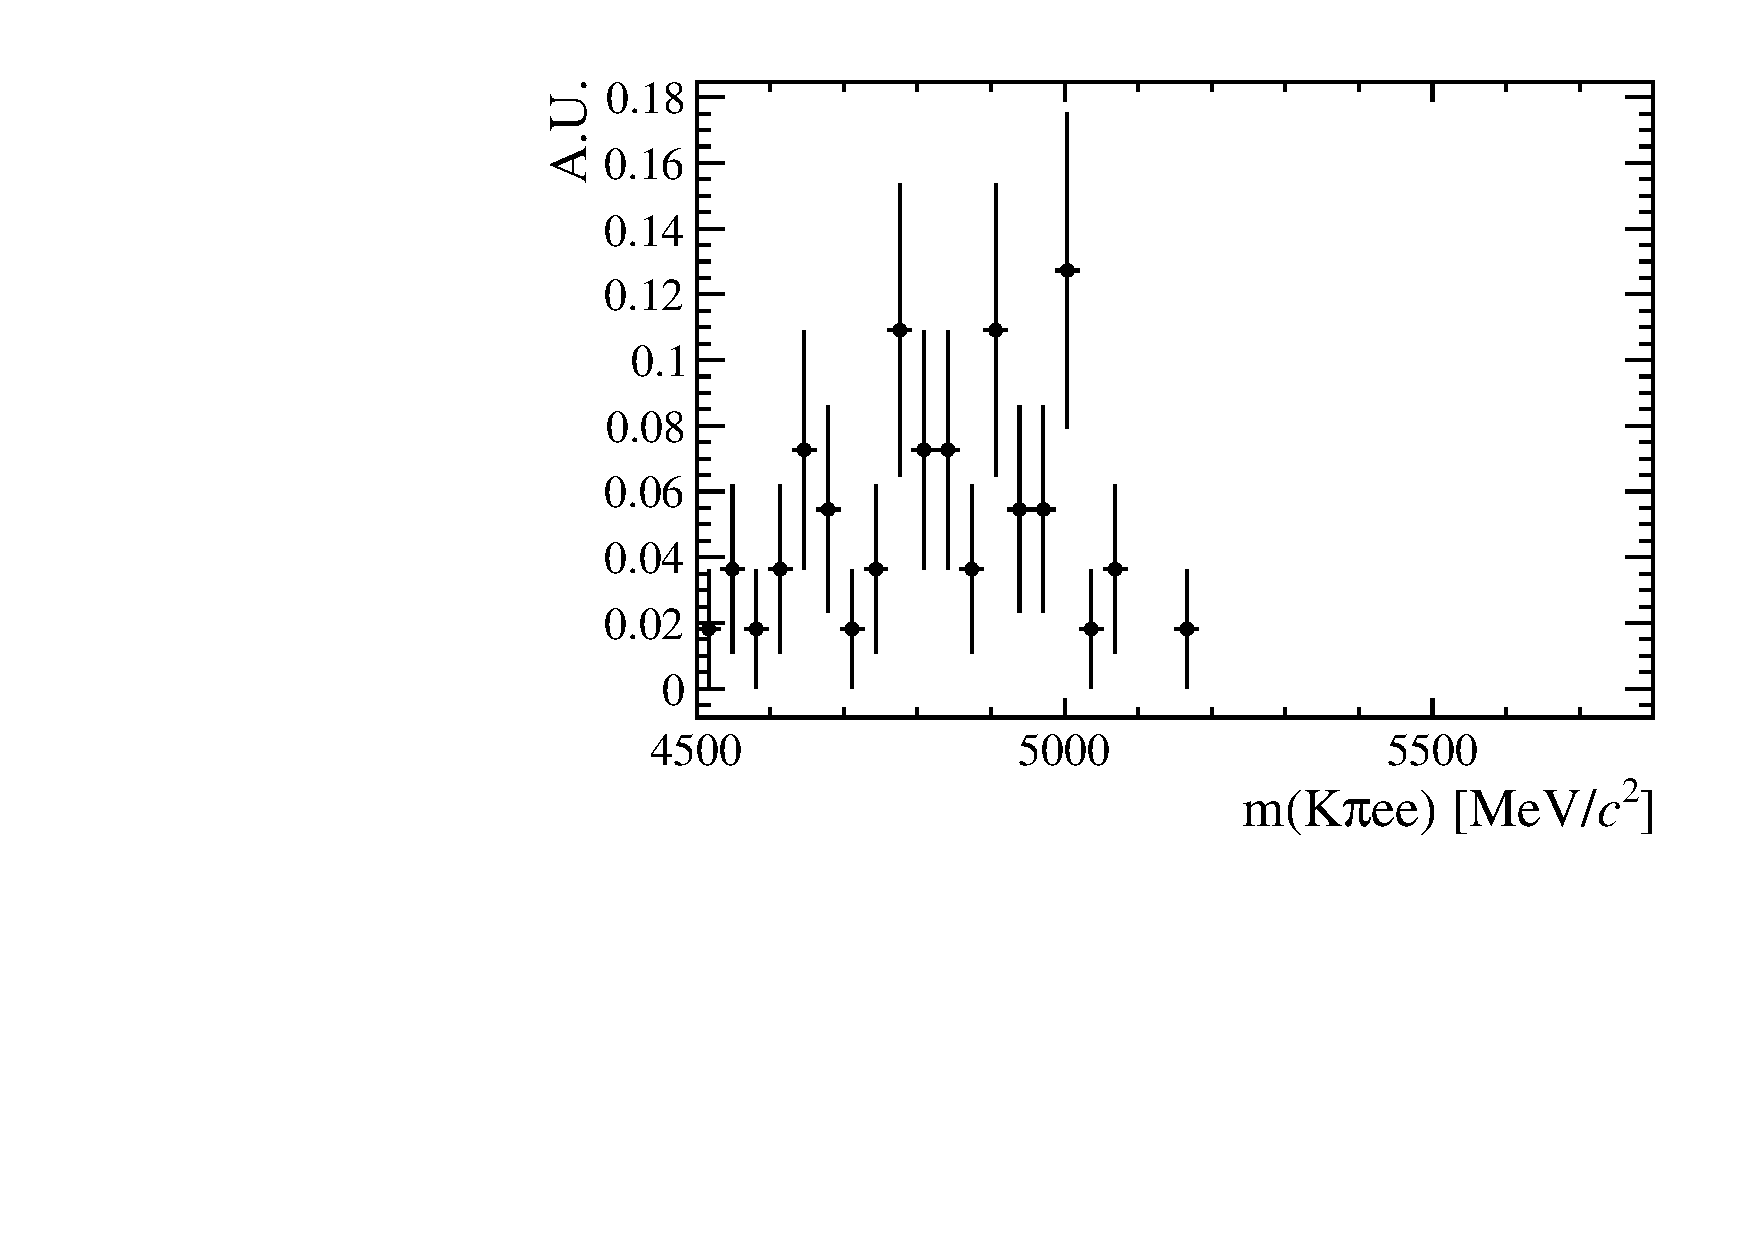
\includegraphics[width=0.48\textwidth]{RKst/figs/misreco/part_had_jpsi.pdf}
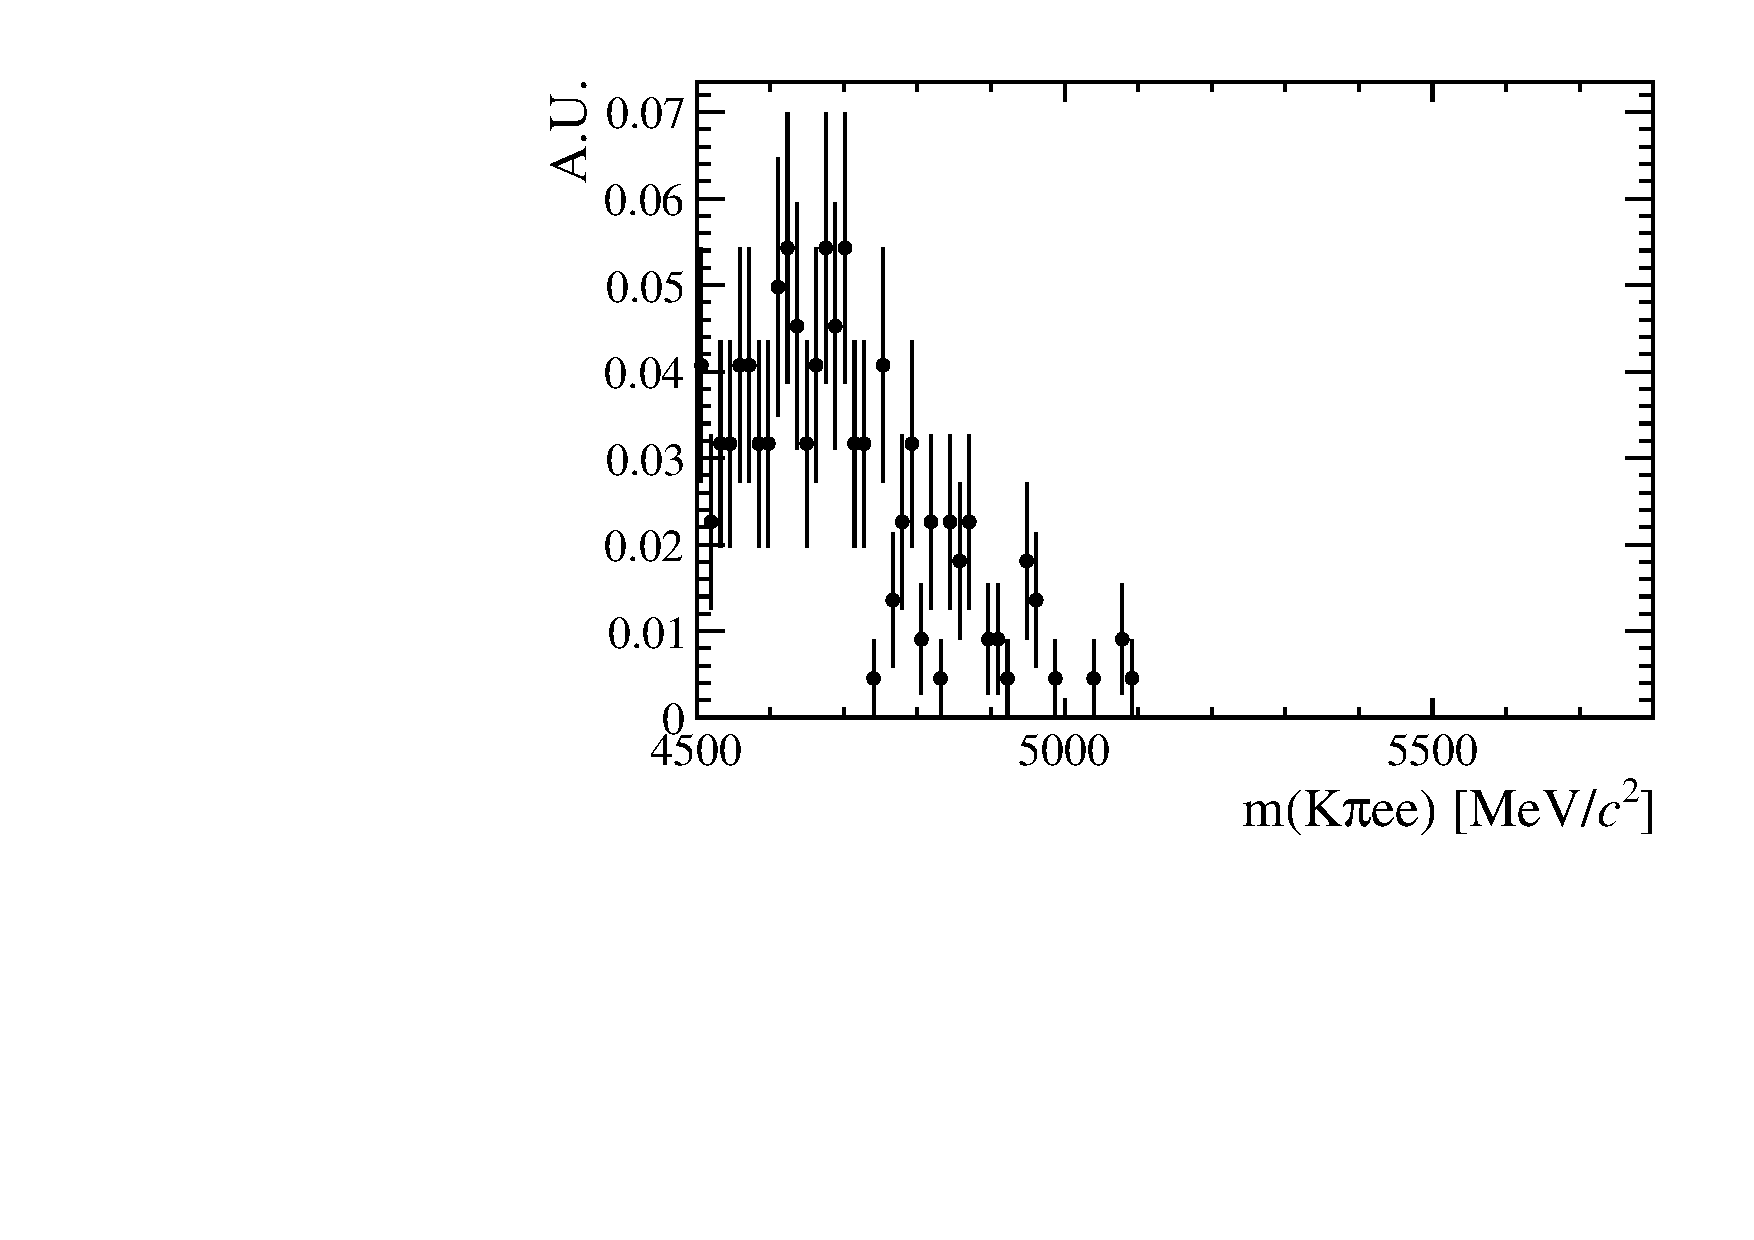
\includegraphics[width=0.48\textwidth]{RKst/figs/misreco/part_lpt_jpsi.pdf}
\caption{Simulated distributions of misreconstructed background events falling into
the $\decay{\Bz}{\Kstar(\jpsi\to\ee)}$ sample coming from the
hadronic (left) and leptonic (right) systems.}
\label{fig:RKst_misreco_distrib}
\end{figure}

In the fit for the rare sample in the central \qsq interval the modelled
backgrounds are: combinatorial background, again modelled with an exponential; misreconstructed background
coming from the hadronic system and the leakage of the \jpsi radiative tail into the lower \qsq interval.
The shape for the misreconstructed component is obtained from simulated distributions similarly to what described
for the resonant channel. However, as there are no inclusive samples for the rare case,
a sample including higher \Kstar resonances is generated, including $K_1^+(1400)$ and $K_2^+(1460)$.
The yield of this component is not floating independently but its relative proportion
with respect to the signal yield is constrained to be the same as in the resonant sample, namely:
\begin{equation}
N_{\ell\ell}^{mis-reco} = N_{ee} \cdot k = N_{ee} \cdot \frac{N_{\jpsi}^{mis-reco}}{N_{\jpsi}}.
\end{equation}
Notice that, as the fit is simultaneous for the rare and resonant samples, this fraction
is not fixed in the fit but floats using information from both samples.

The shape to describe the \jpsi tail leakage is obtained using simulated $\Bz\to\jpsi\Kstar$ candidates
and selecting those falling in \qsq below 6 \gevgevcccc. The 4-body invariant mass distribution
of these events is reported in Fig.~\ref{fig:RKst_rare_misreco_distrib}. The yield of this component
again is not floating independently but it is liked to the yield found in the resonant fit as follows
\begin{equation}
N_{\ell\ell}^{leak} = N_{\jpsi} \cdot k^{MC} = N_{\jpsi} \cdot \frac{N_{leak}^{MC}}{N_{\jpsi}^{MC}}
\end{equation}
where $k$ is the ratio between $N_{\jpsi}^{MC}$, the number of \jpsi events
that fall into the \jpsi ~\qsq window (6-11 \gevgevcccc) in the simulation
and $N_{leak}^{MC}$, the number of \jpsi events leaking below 6 \gevgevcccc in the simulation.
In this case $k$ is previously extracted from simulated events and fixed in the fit on data.

\begin{figure}[h!]
\centering
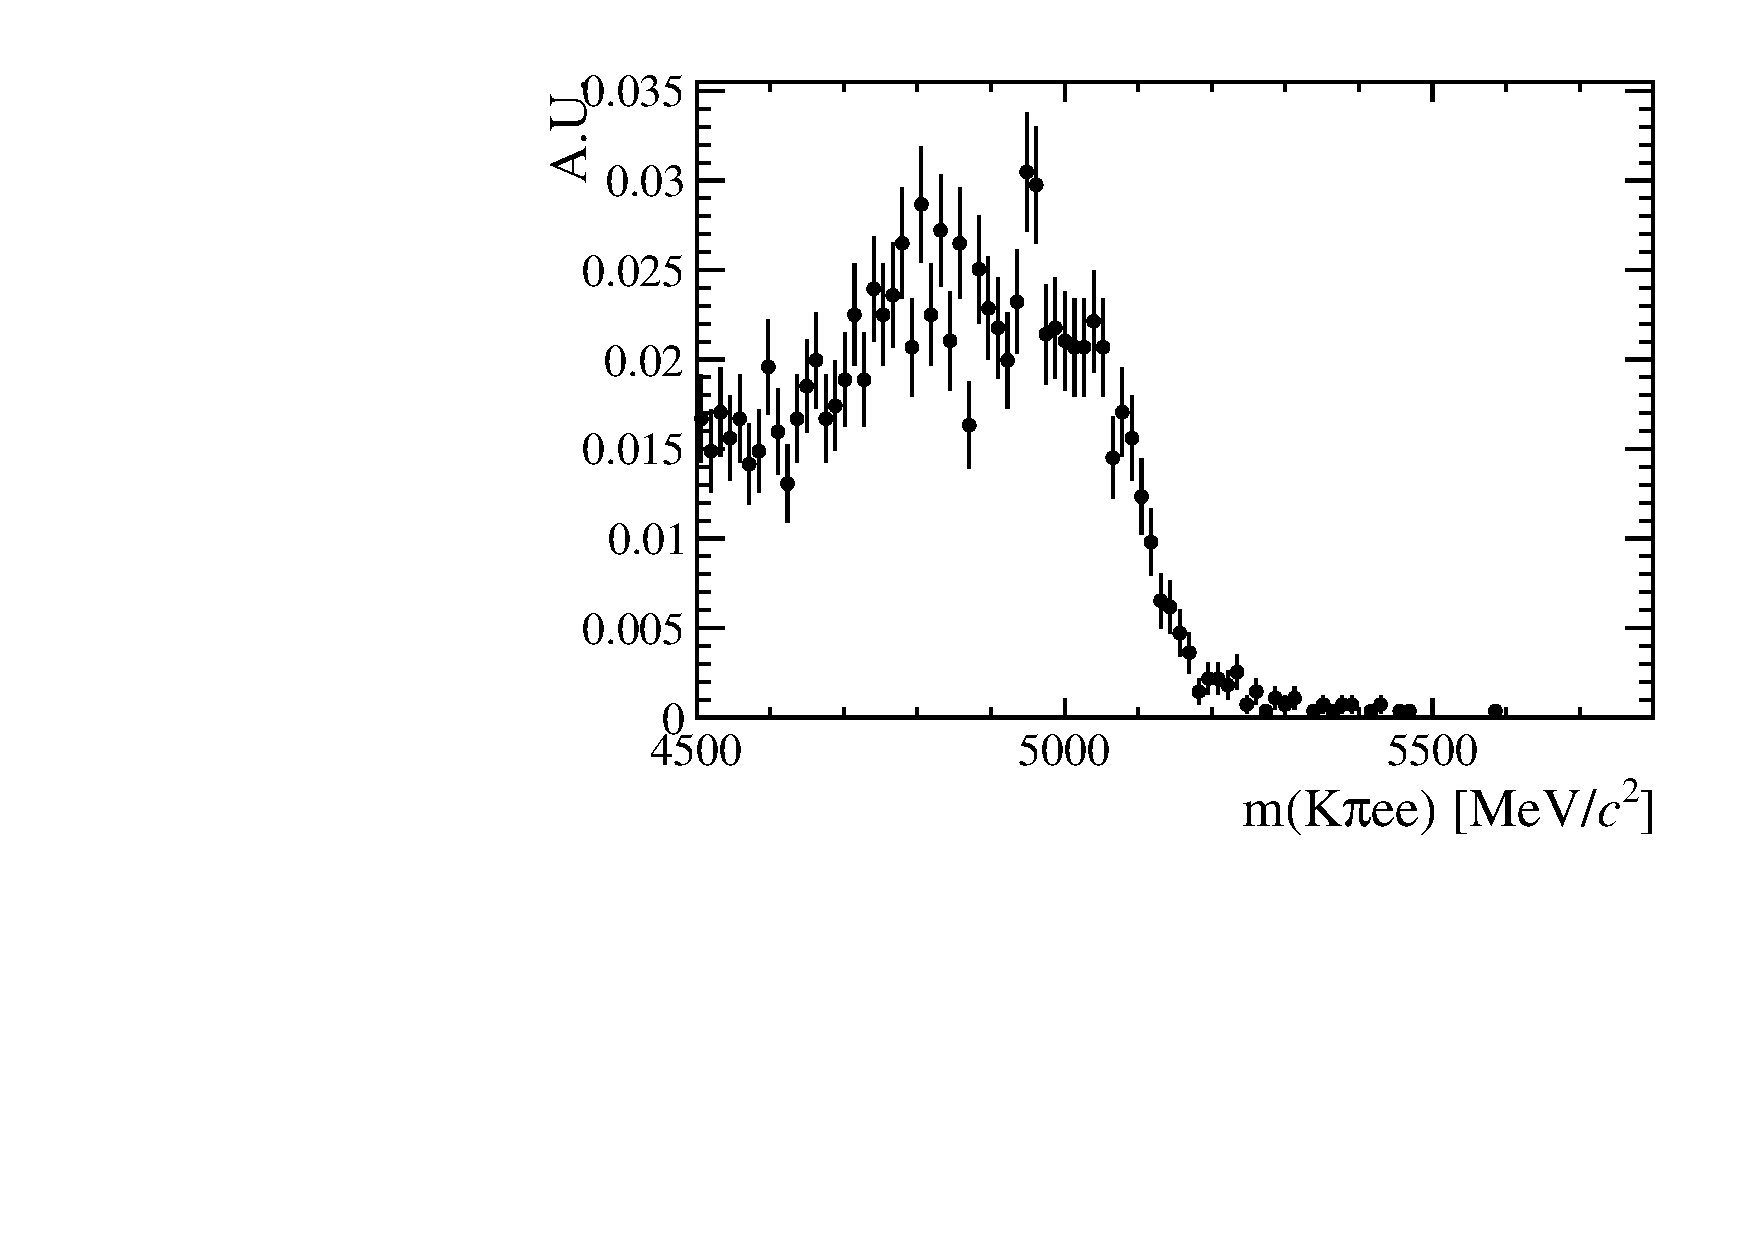
\includegraphics[width=0.48\textwidth]{RKst/figs/misreco/part_had.pdf}
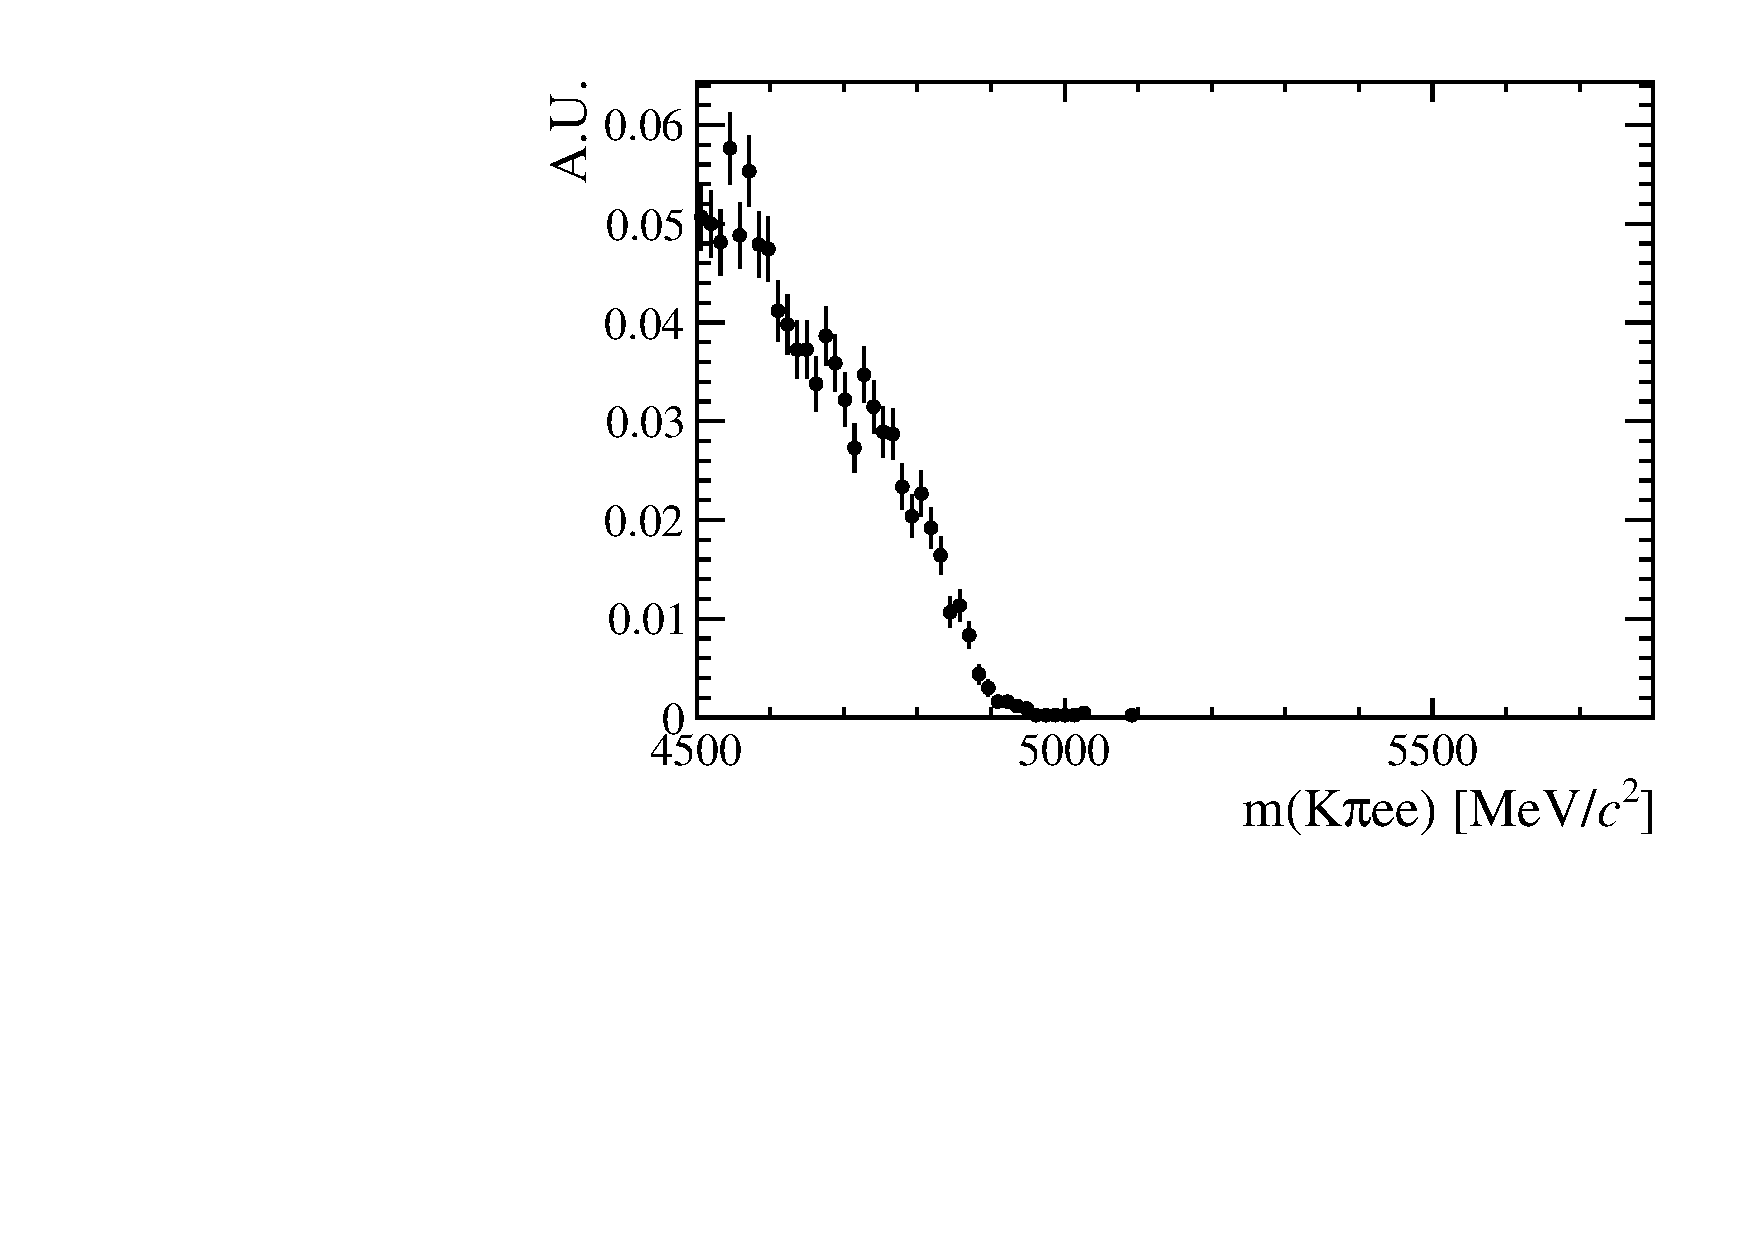
\includegraphics[width=0.48\textwidth]{RKst/figs/misreco/jpsi_leakage.pdf}
\caption{(left) Simulated 4-body invariant mass distributions for events involving
higher \Kstar states and passing out full selection. (right) Simulated invariant mass
distribution of $\decay{\Bz}{\Kstar(\jpsi\to\ee)}$ events leaking into the central \qsq interval.}
\label{fig:RKst_rare_misreco_distrib}
\end{figure}


\subsection{Summary of the fit to electronic channels in the central \qsq interval}

In summary in the resonant fit on data the floating parameters are the yields of all the components
in the resonant channel, a common $R_{ee}$ ratio, the combinatorial background yield in the rare sample,
one scale factor $c$, one mass shift $m_0$ and the combinatorial background slopes.

In Fig.~\ref{fig:FitEE_MC_inTrigCat_Brem0} are reported fits on simulated $\Bz\to\Kstar(\jpsi\to\ee)$ candidates for
all trigger categories and no photons emitted, in Fig.~\ref{fig:FitEE_MC_inTrigCat_Brem1} for one photon emitted
and in Fig.~\ref{fig:FitEE_MC_inTrigCat_Brem2} for two photons emitted. Finally, in
Fig.~\ref{fig:FitJpsiEE_Data_inTrigCat} and \ref{fig:FitEE_Data_inTrigCat} are reported fits
on real $\Bz\to\Kstar(\jpsi\to\ee)$ and $\Bz\to\Kstar \ee$ candidates (1.1--6 \gevgevcccc interval)
in the three trigger categories. Values of fitted parameters are reported on the plots.

\begin{figure}[h!]
\centering
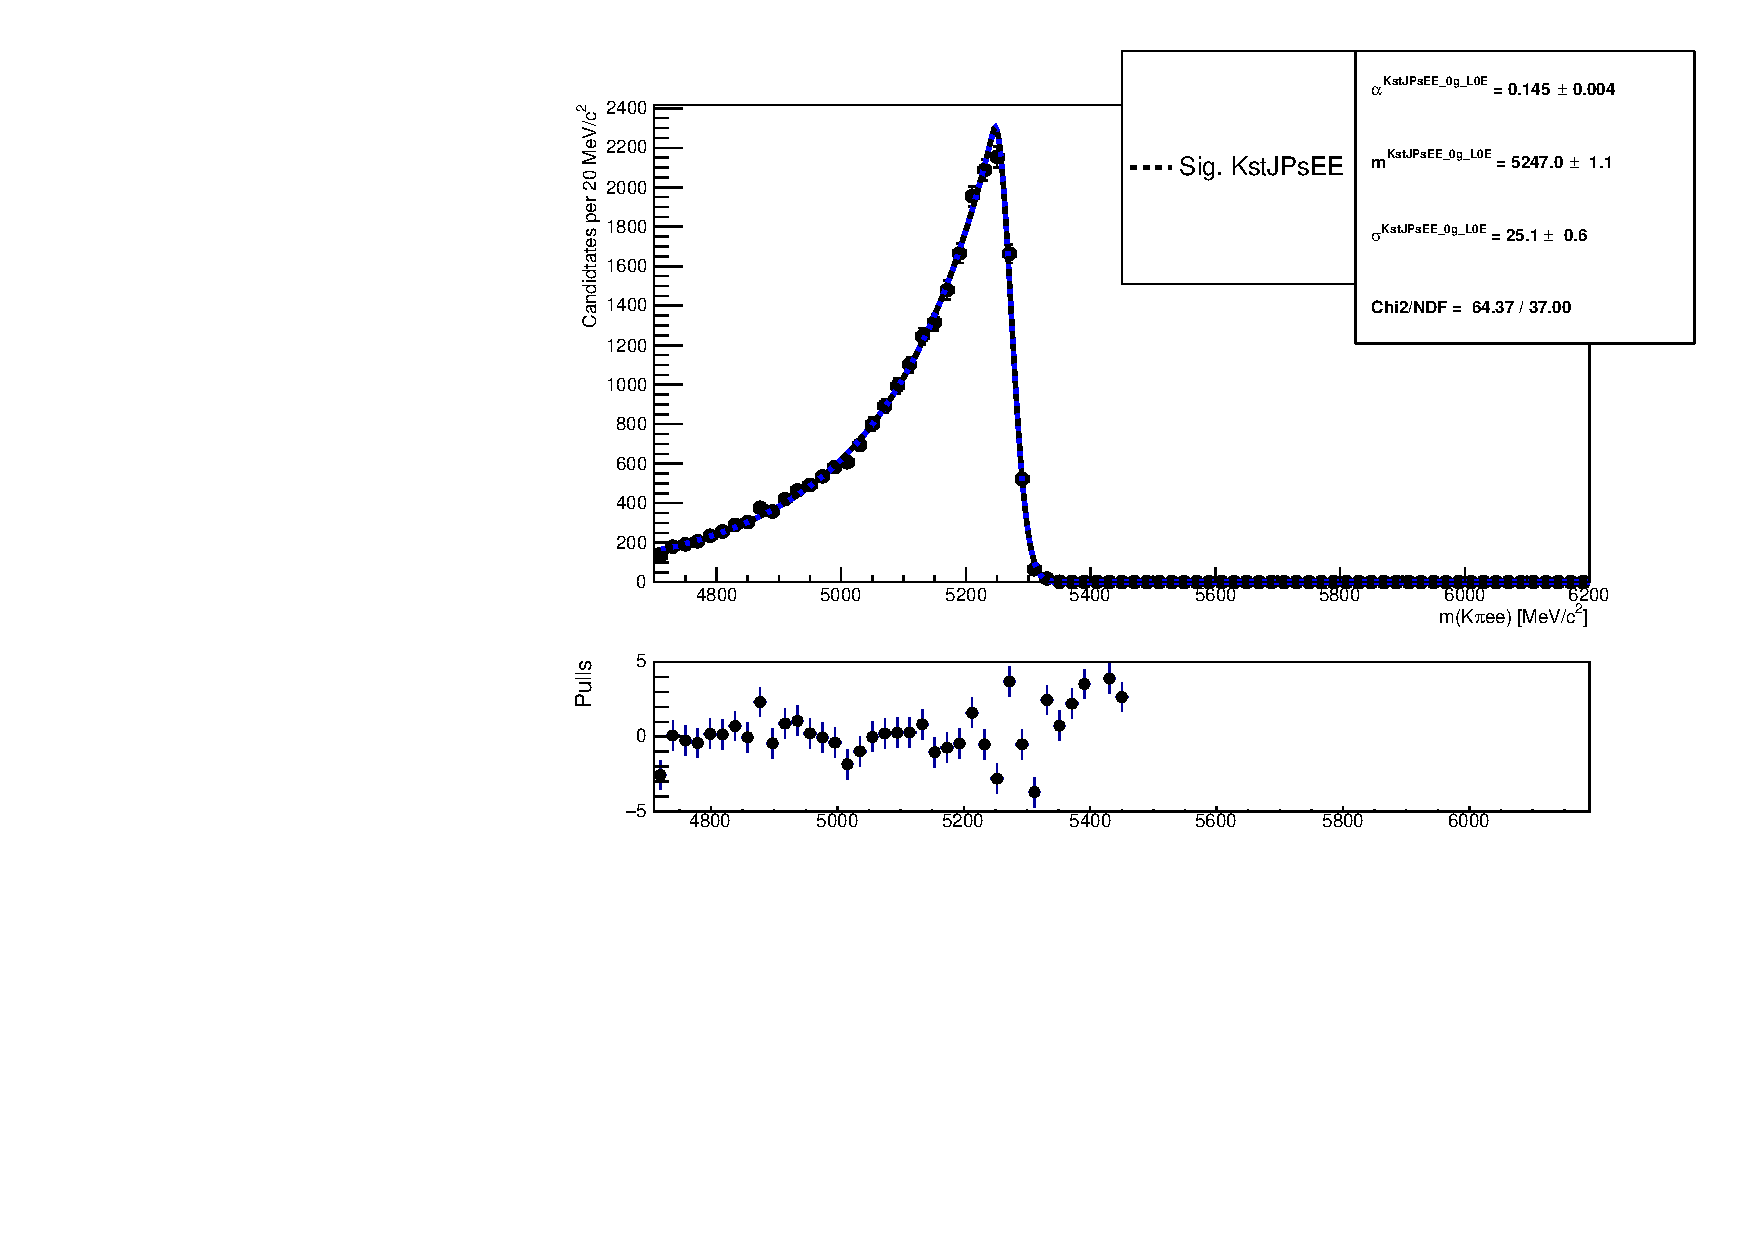
\includegraphics[width=0.40\textwidth]{RKst/figs/fit_EEs_0_EE-q2central-gmc/KstJPsEE_0g_L0E_fitAndRes.pdf}
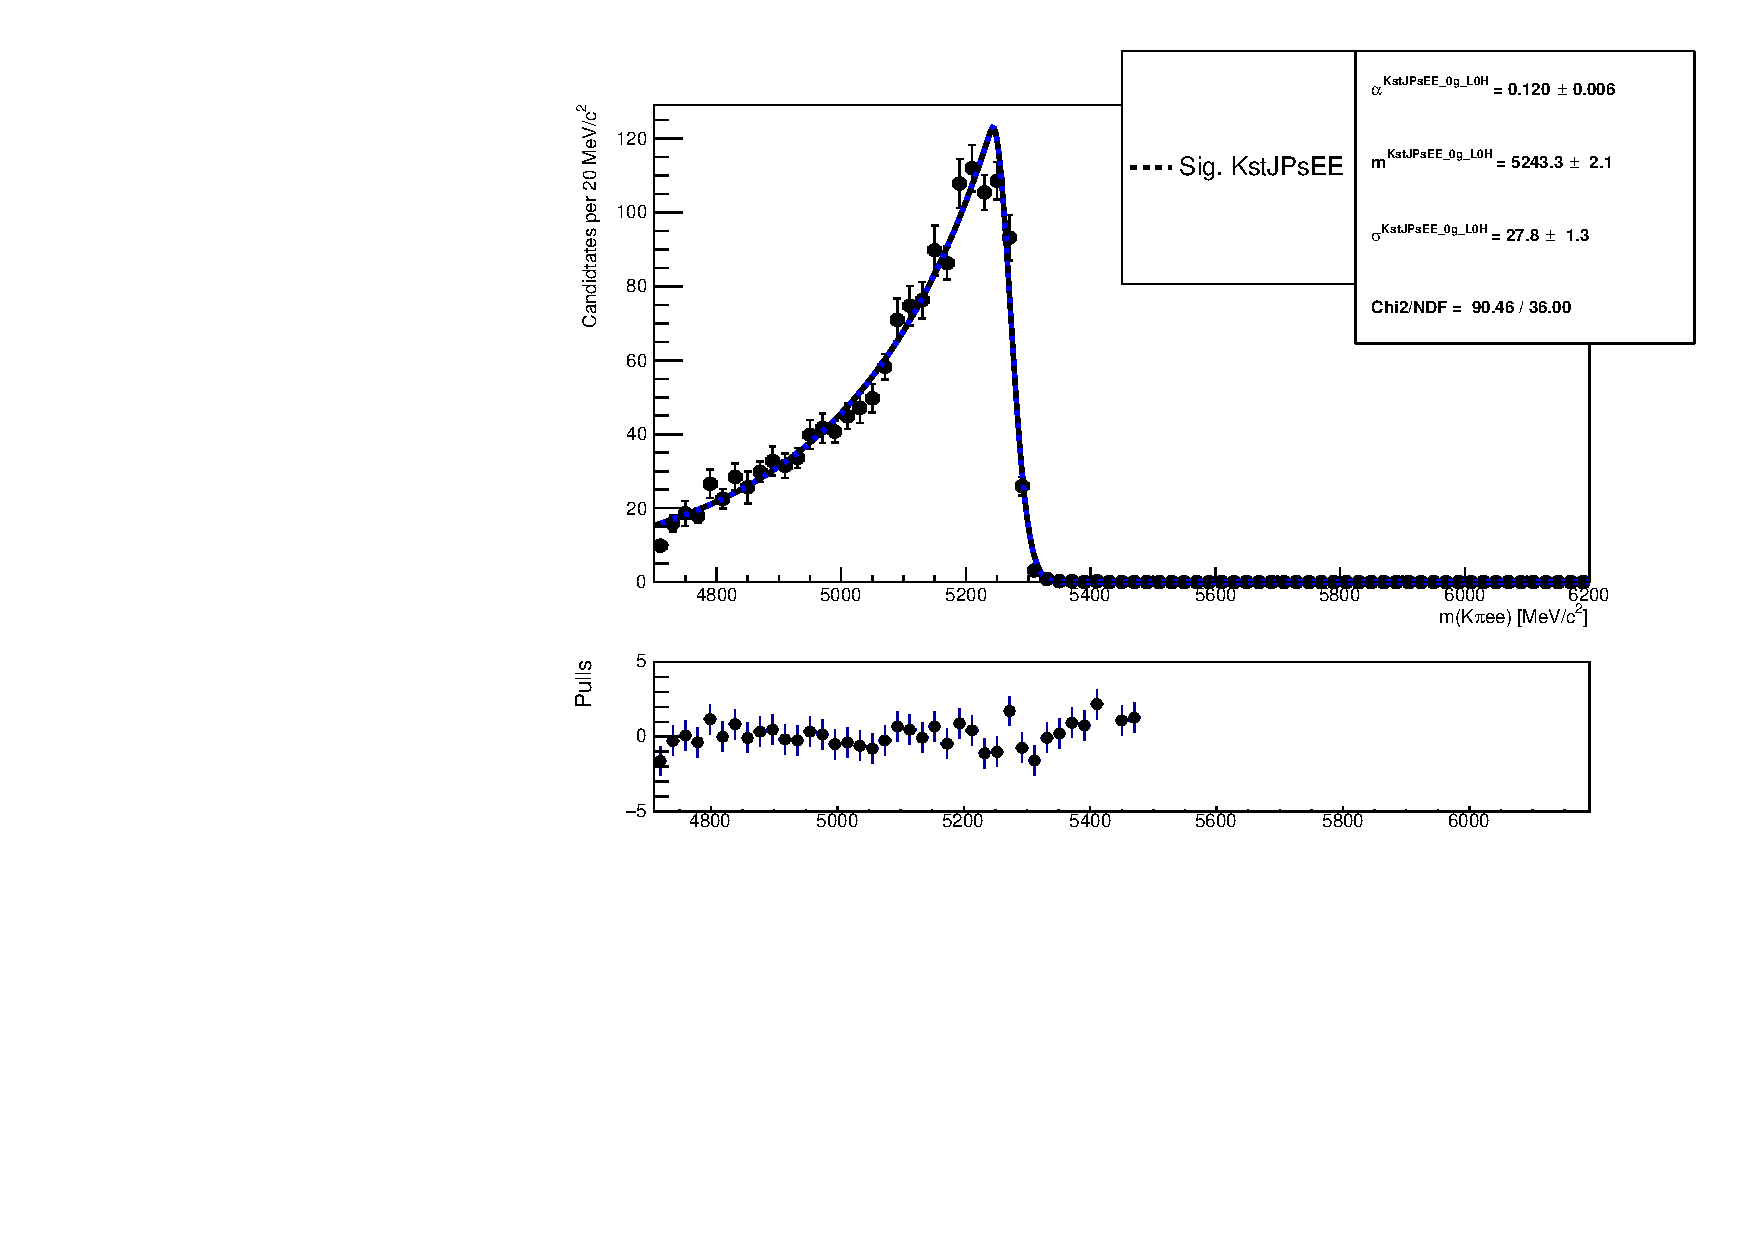
\includegraphics[width=0.40\textwidth]{RKst/figs/fit_EEs_0_EE-q2central-gmc/KstJPsEE_0g_L0H_fitAndRes.pdf}
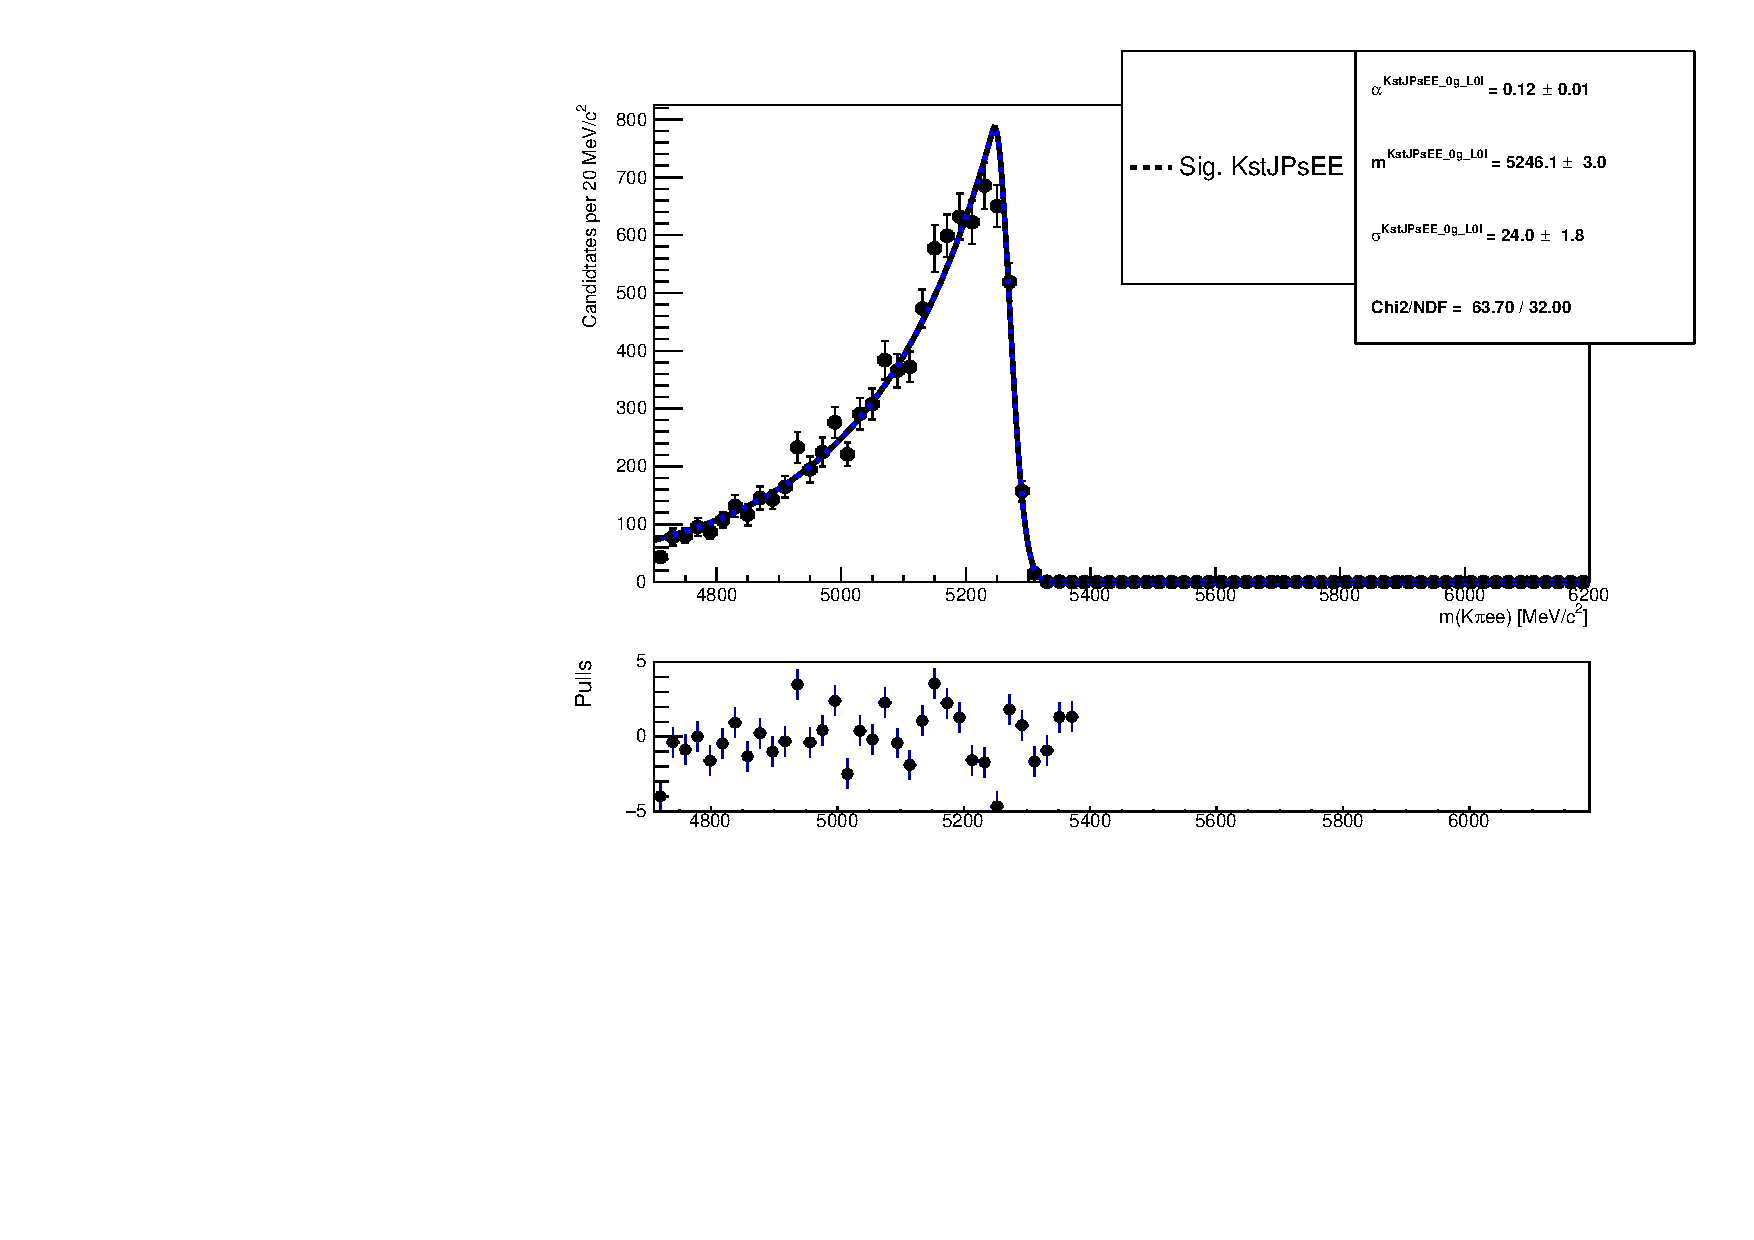
\includegraphics[width=0.40\textwidth]{RKst/figs/fit_EEs_0_EE-q2central-gmc/KstJPsEE_0g_L0I_fitAndRes.pdf}
\caption{Fitted $m(K\pi ee)$ mass spectrum of $B^0 \rightarrow K^{*0} J/\psi(J/\psi\rightarrow ee)$ simulated
events in the three trigger categories and no photon emitted. }
\label{fig:FitEE_MC_inTrigCat_Brem0}
\end{figure}
%
%\clearpage
\begin{figure}[h!]
\centering
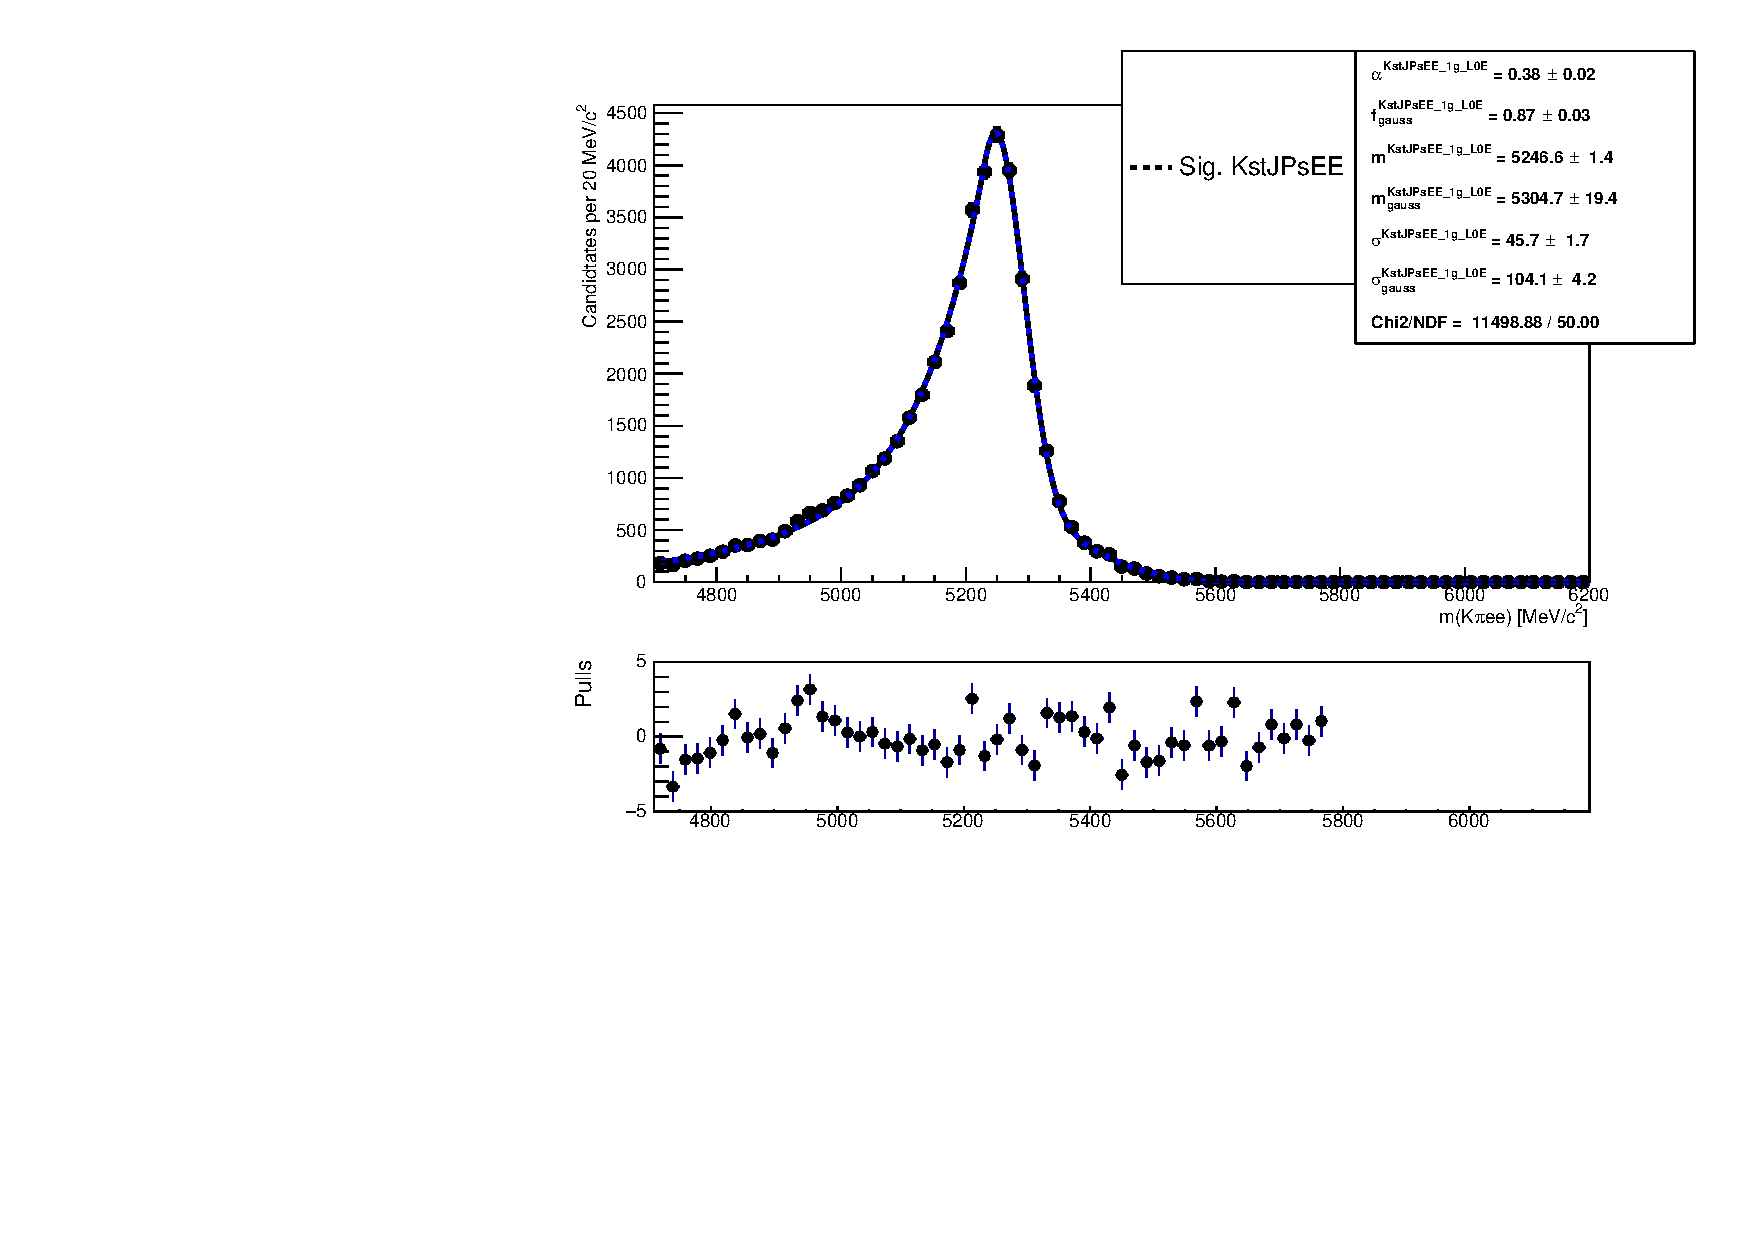
\includegraphics[width=0.46\textwidth]{RKst/figs/fit_EEs_0_EE-q2central-gmc/KstJPsEE_1g_L0E_fitAndRes.pdf}
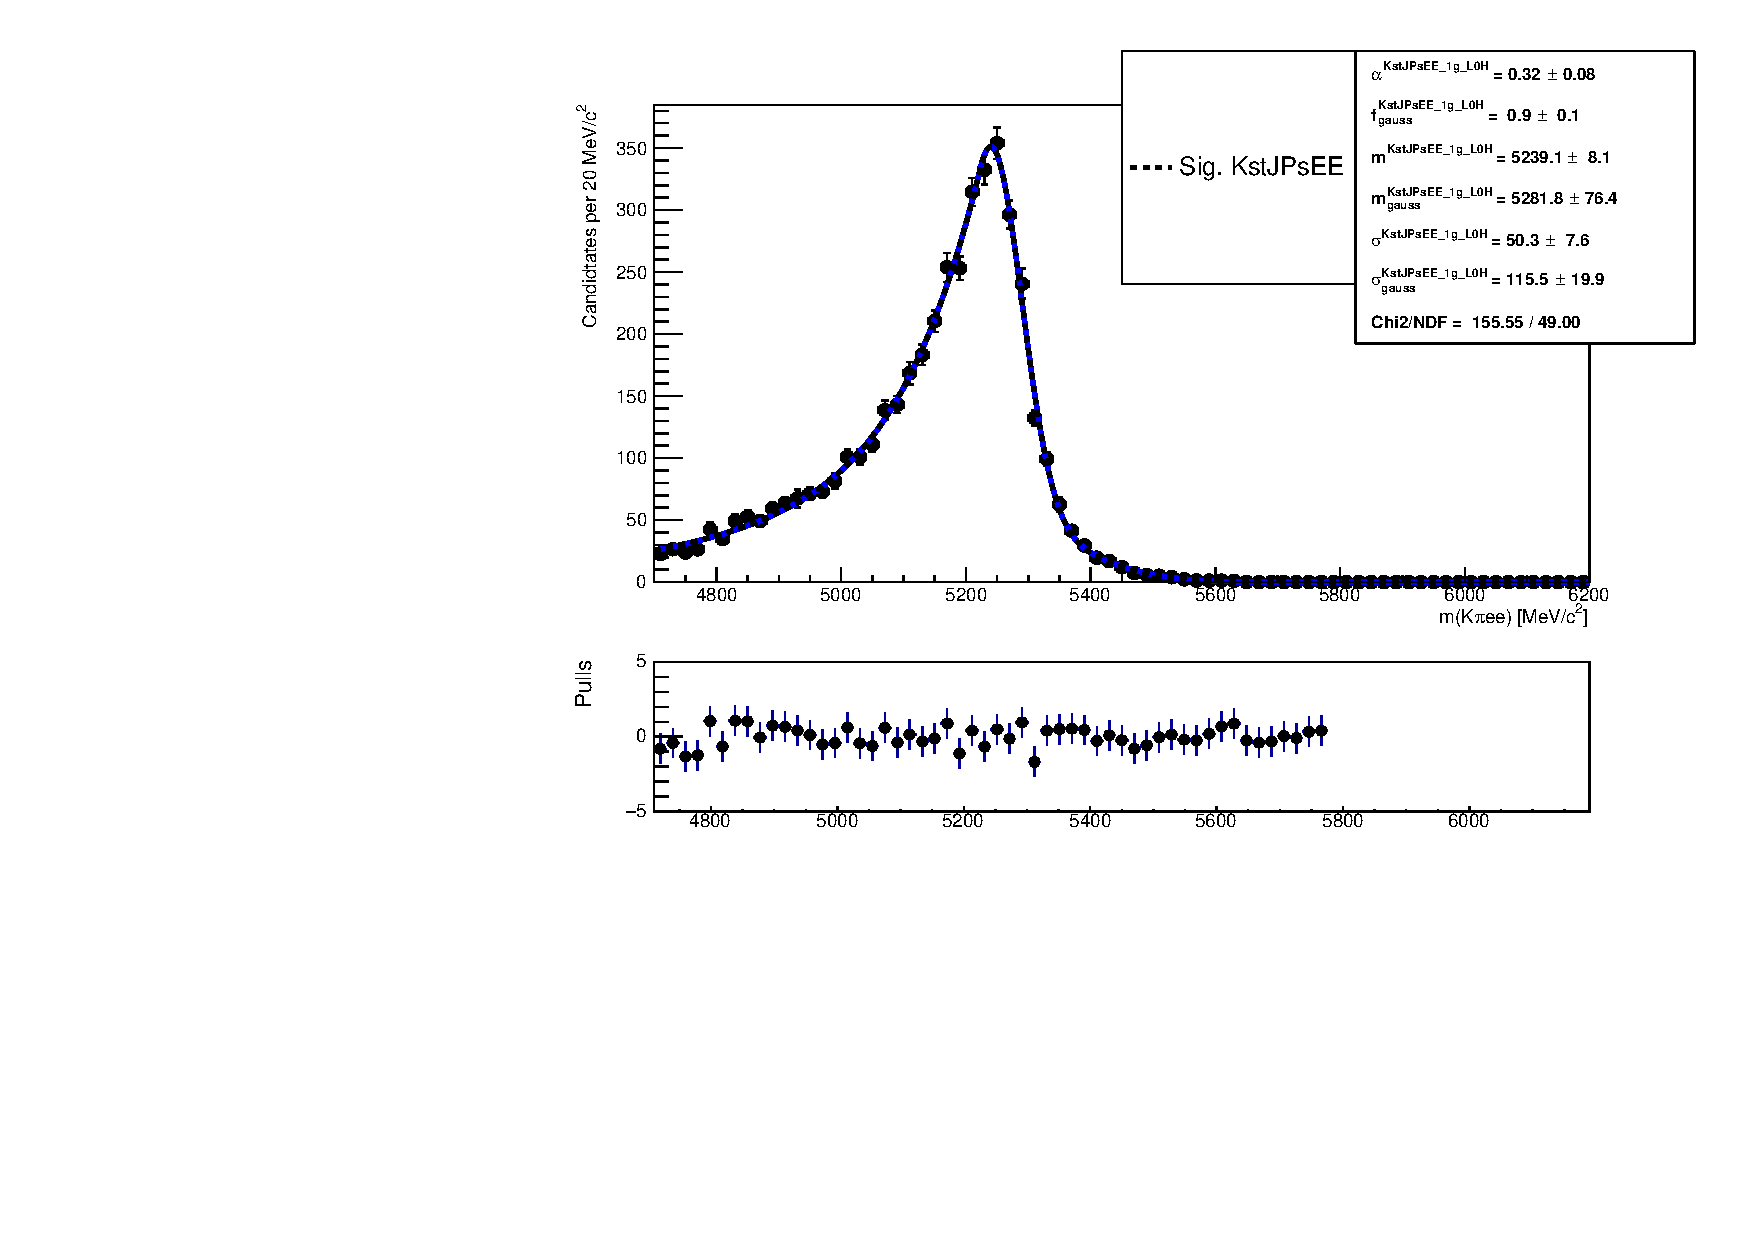
\includegraphics[width=0.46\textwidth]{RKst/figs/fit_EEs_0_EE-q2central-gmc/KstJPsEE_1g_L0H_fitAndRes.pdf}
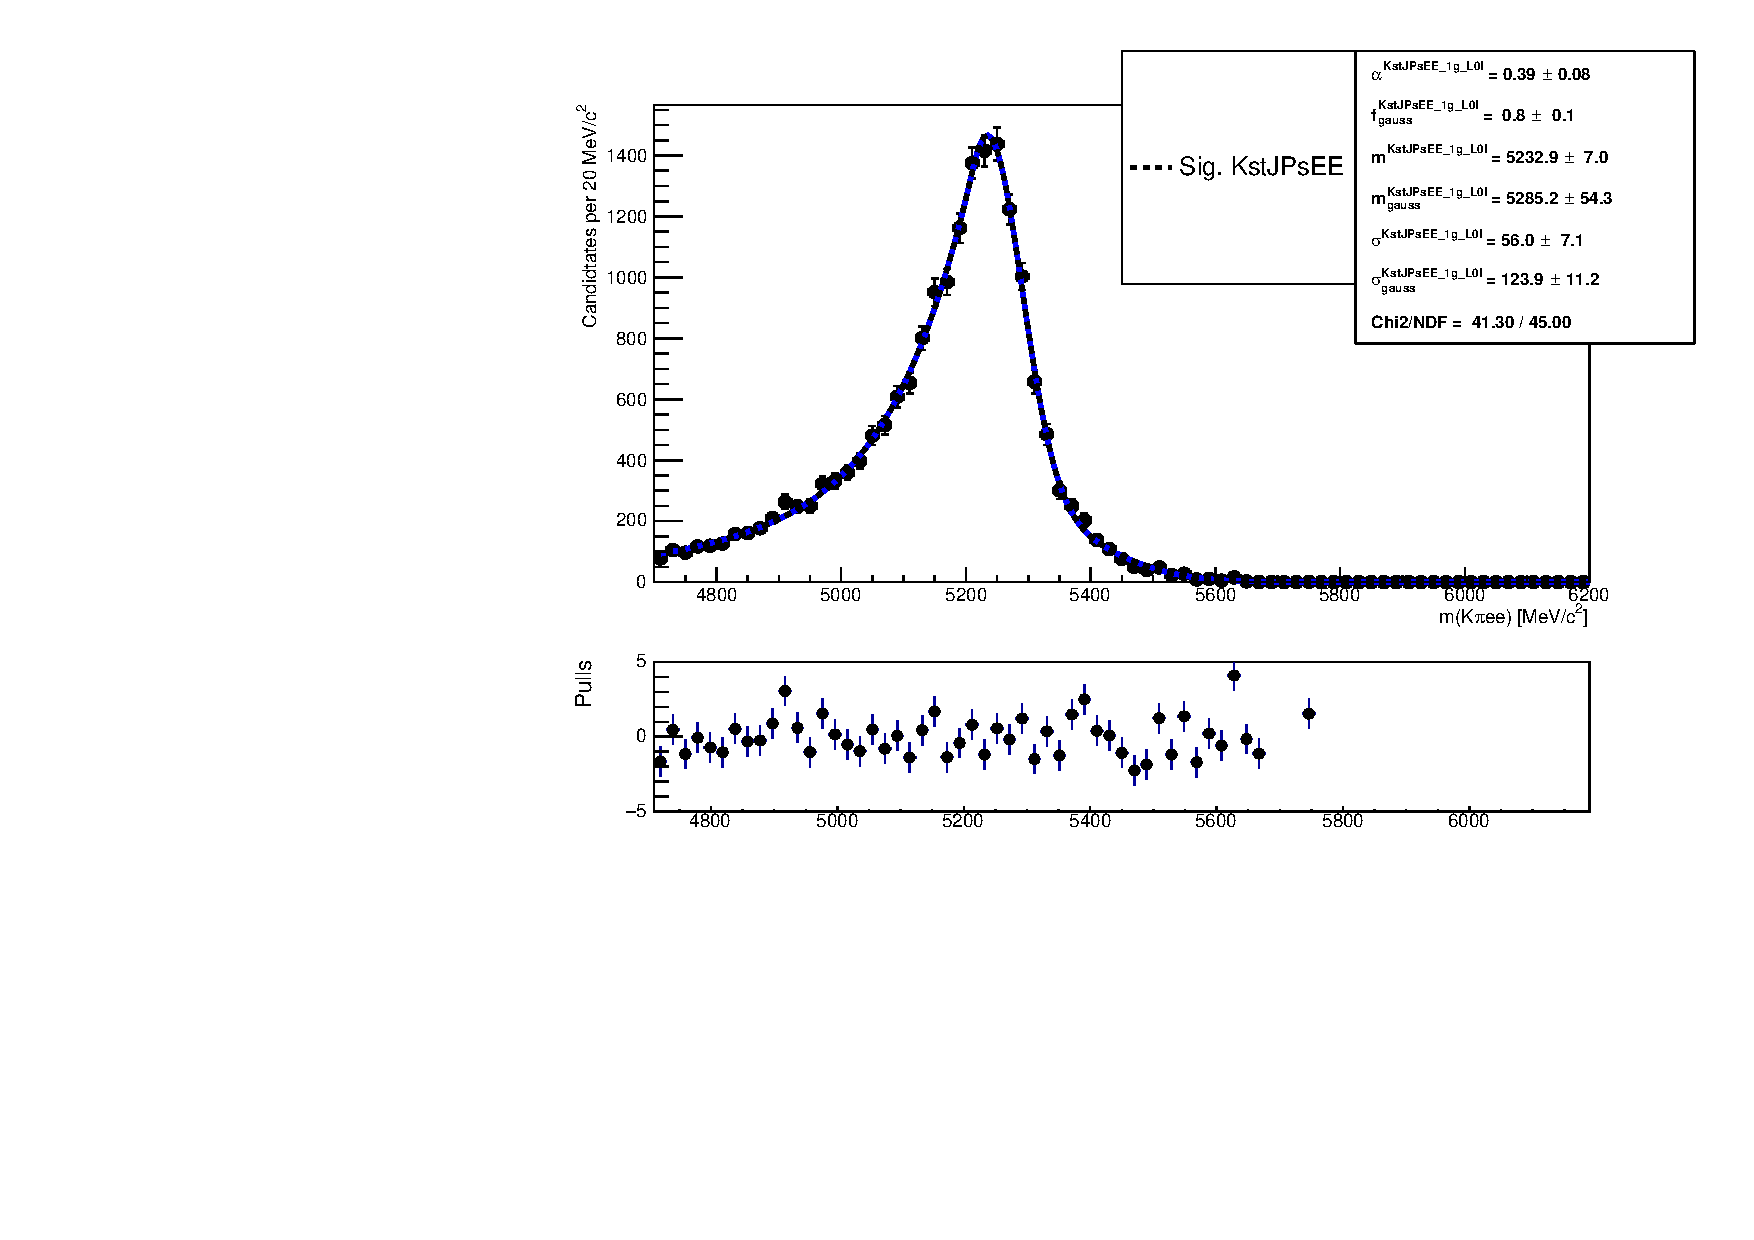
\includegraphics[width=0.46\textwidth]{RKst/figs/fit_EEs_0_EE-q2central-gmc/KstJPsEE_1g_L0I_fitAndRes.pdf}
\caption{Fitted $m(K\pi ee)$ mass spectrum of $B^0 \rightarrow K^{*0} J/\psi(J/\psi\rightarrow ee)$ simulated
events in the three trigger categories and one photon emitted. }
\label{fig:FitEE_MC_inTrigCat_Brem1}
\end{figure}
%
\begin{figure}[h!]
\centering
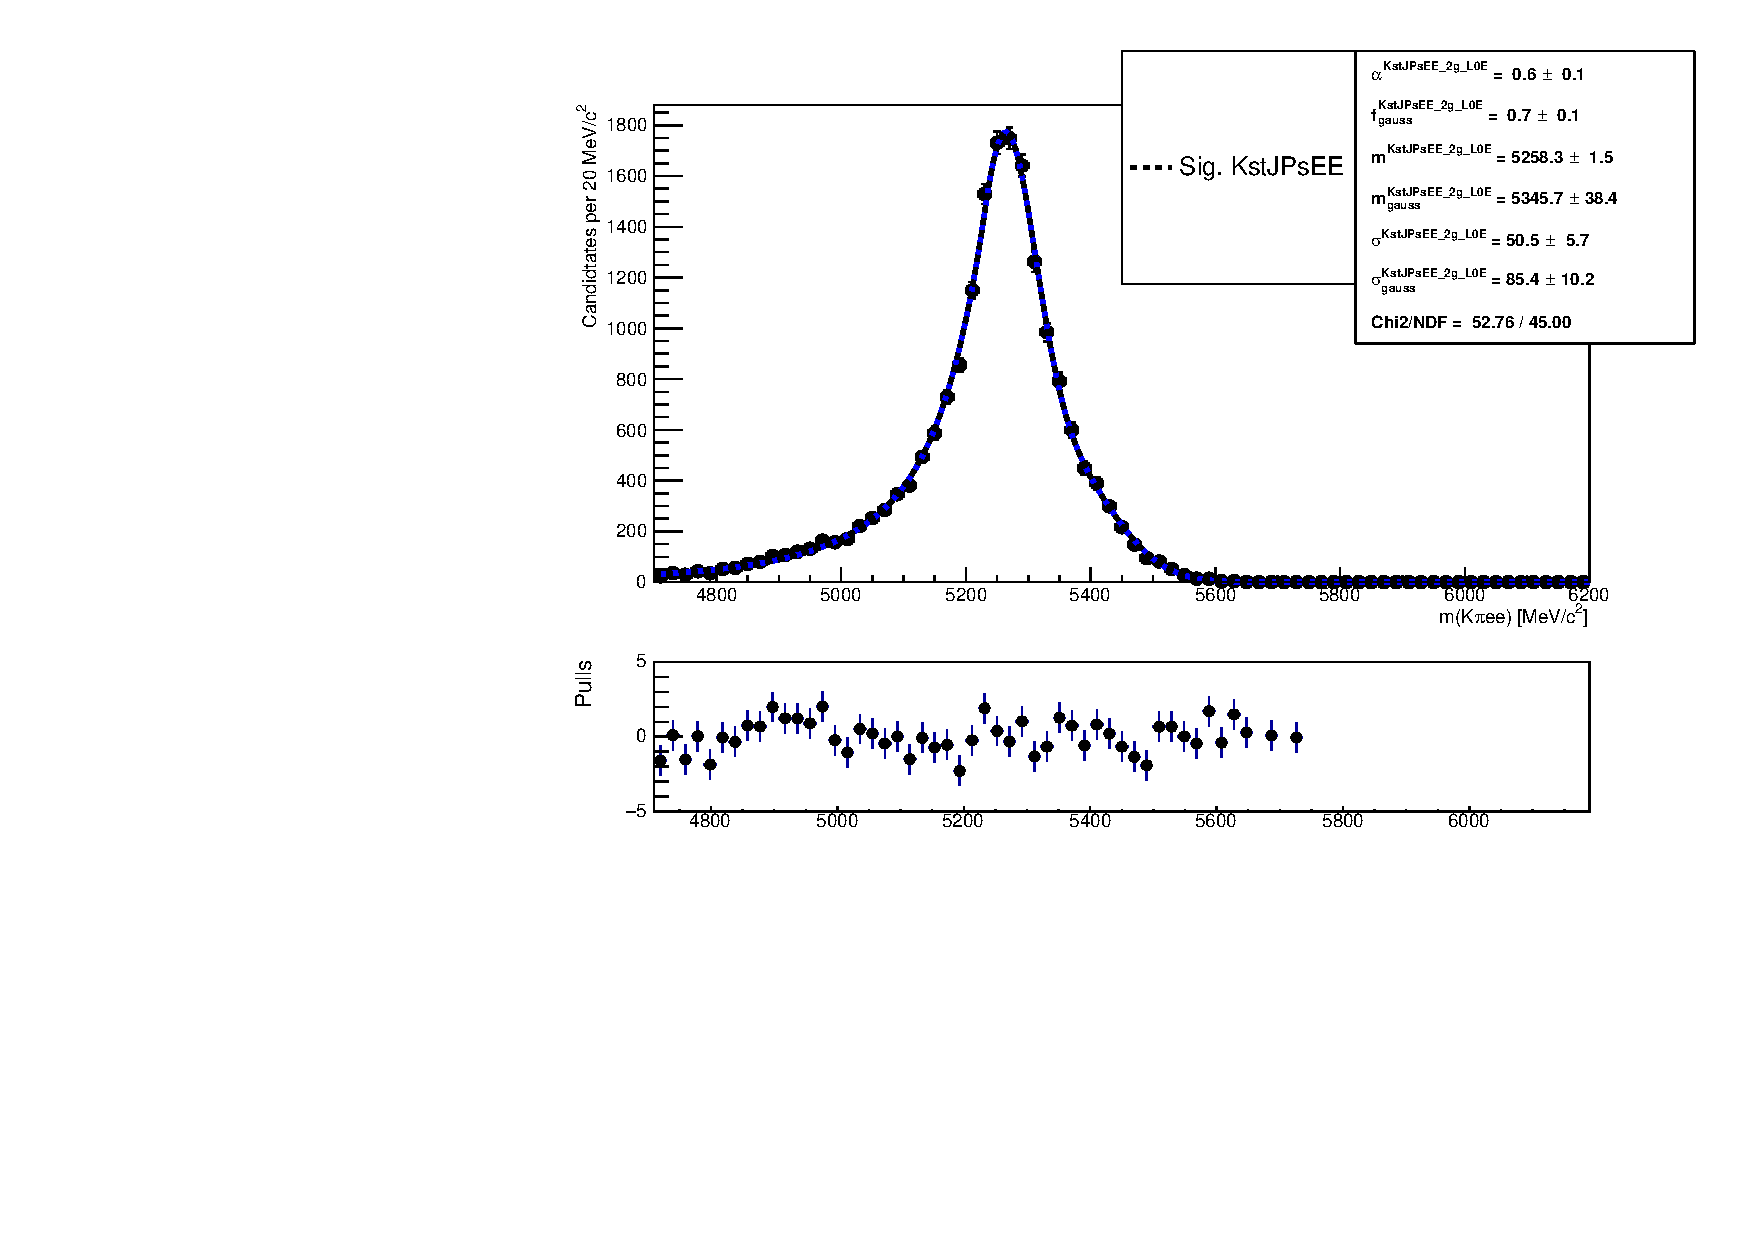
\includegraphics[width=0.46\textwidth]{RKst/figs/fit_EEs_0_EE-q2central-gmc/KstJPsEE_2g_L0E_fitAndRes.pdf}
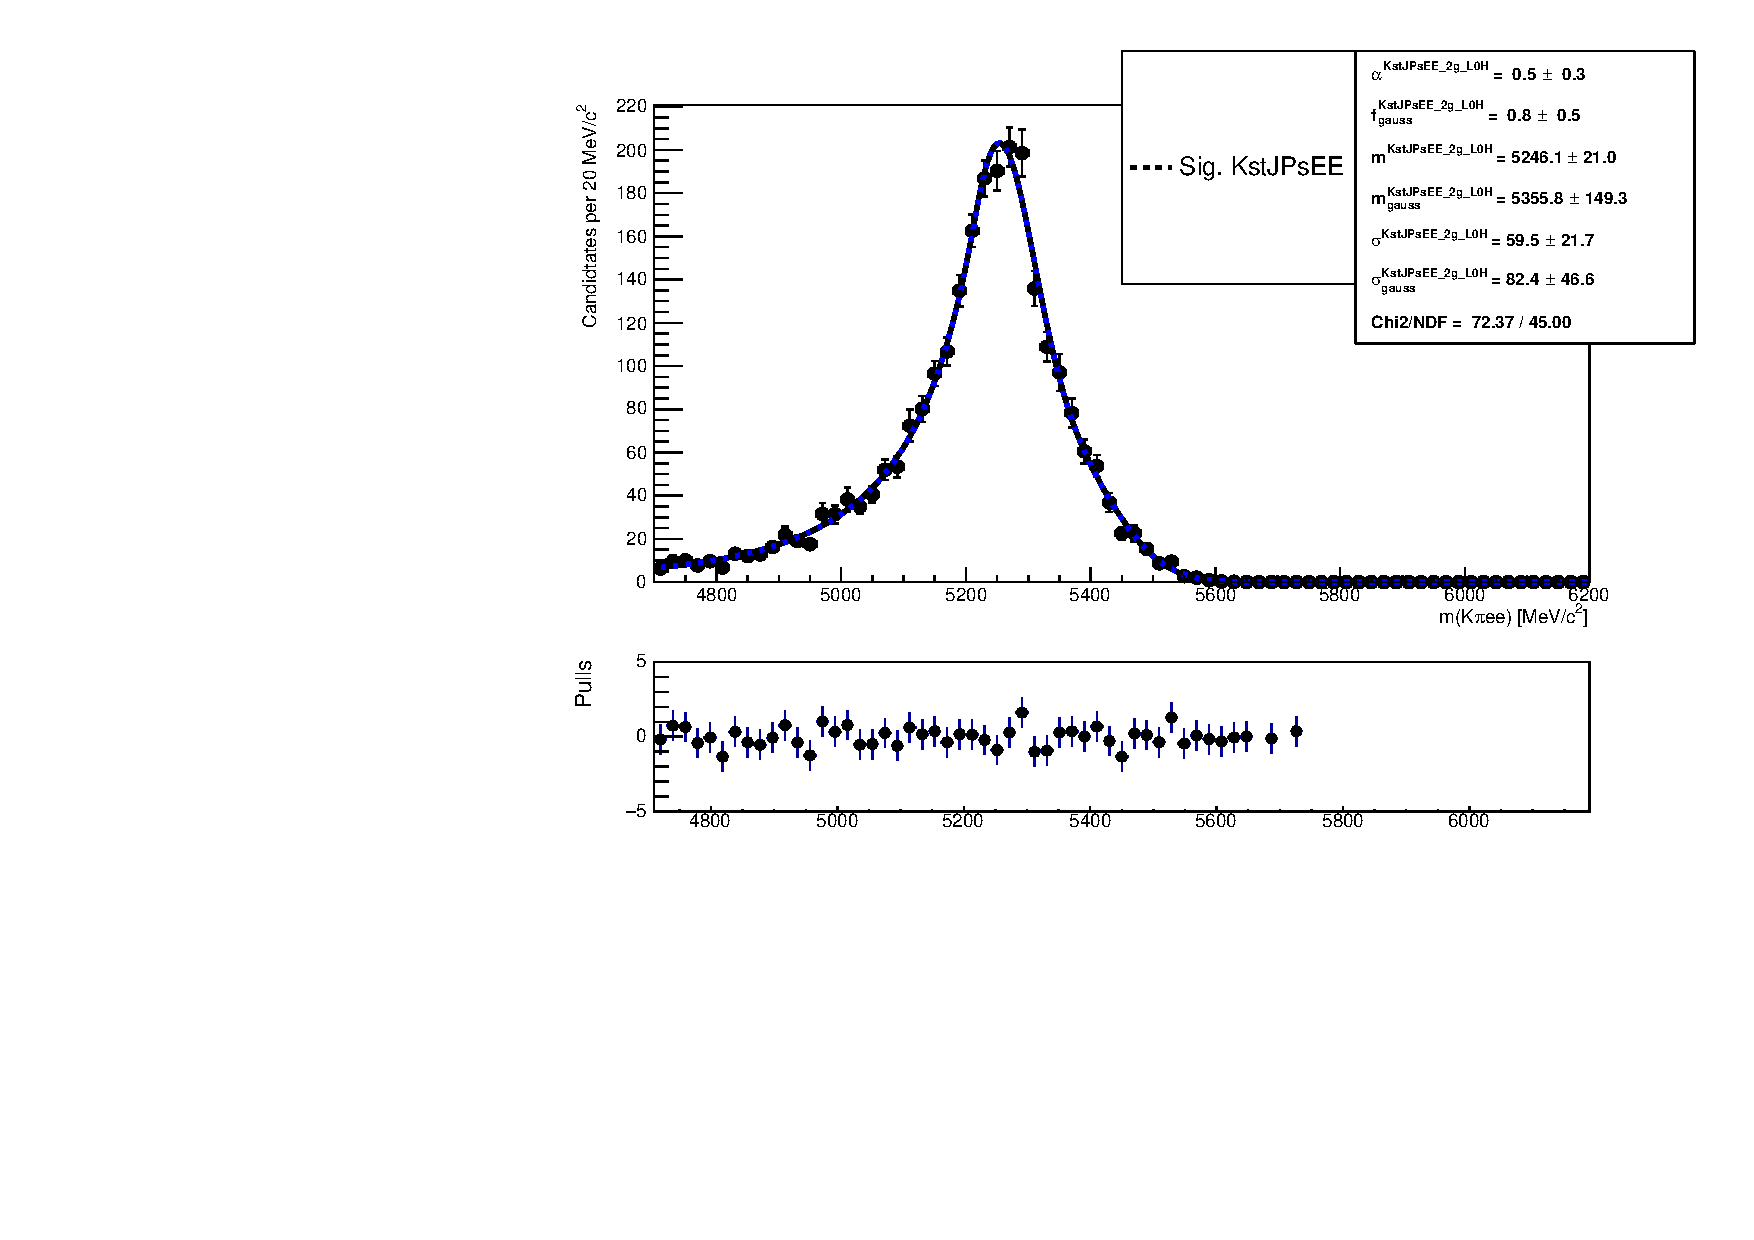
\includegraphics[width=0.46\textwidth]{RKst/figs/fit_EEs_0_EE-q2central-gmc/KstJPsEE_2g_L0H_fitAndRes.pdf}
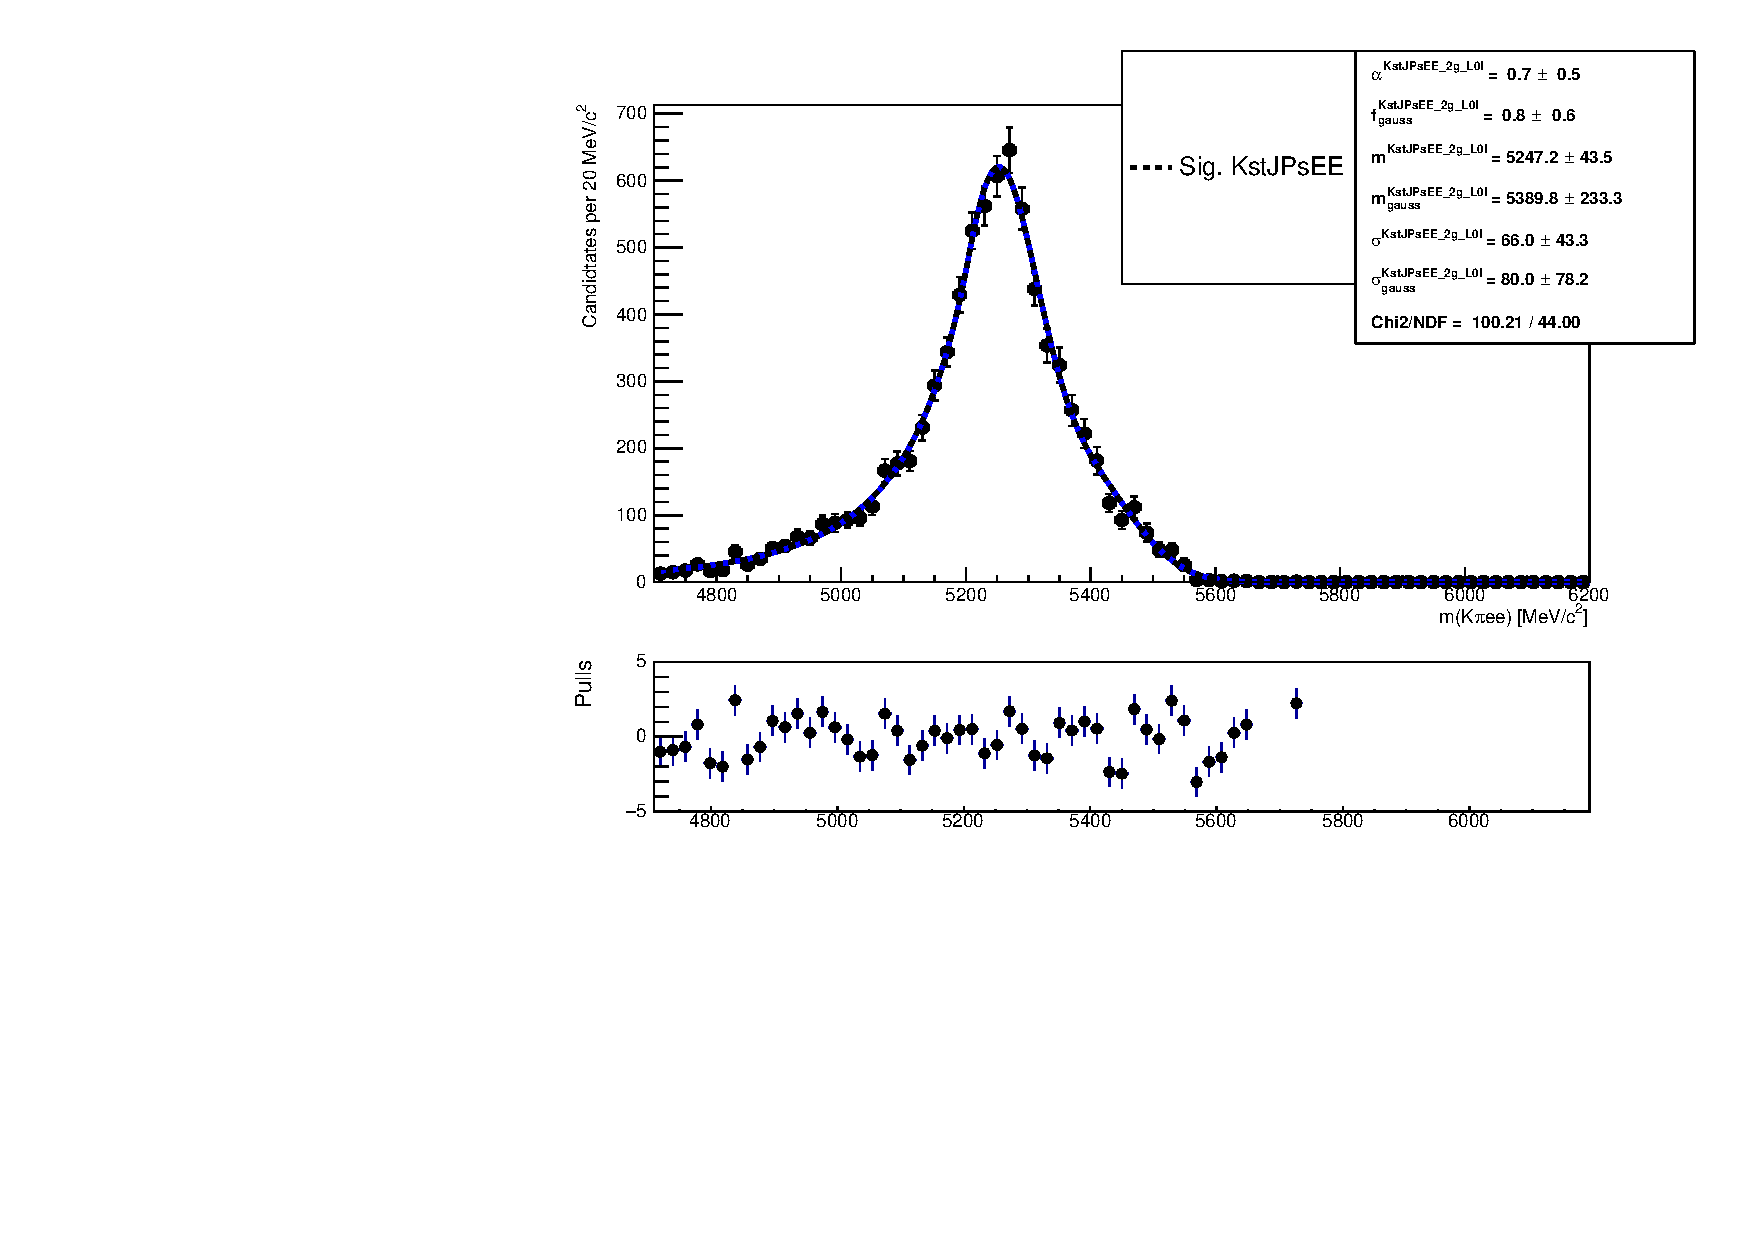
\includegraphics[width=0.46\textwidth]{RKst/figs/fit_EEs_0_EE-q2central-gmc/KstJPsEE_2g_L0I_fitAndRes.pdf}
\caption{Fitted $m(K\pi ee)$ mass spectrum of $B^0 \rightarrow K^{*0} J/\psi(J/\psi\rightarrow ee)$ simulated
events in the three trigger categories and two photons emitted. }
\label{fig:FitEE_MC_inTrigCat_Brem2}
\end{figure}
%
%\clearpage
\begin{figure}[h!]
\centering
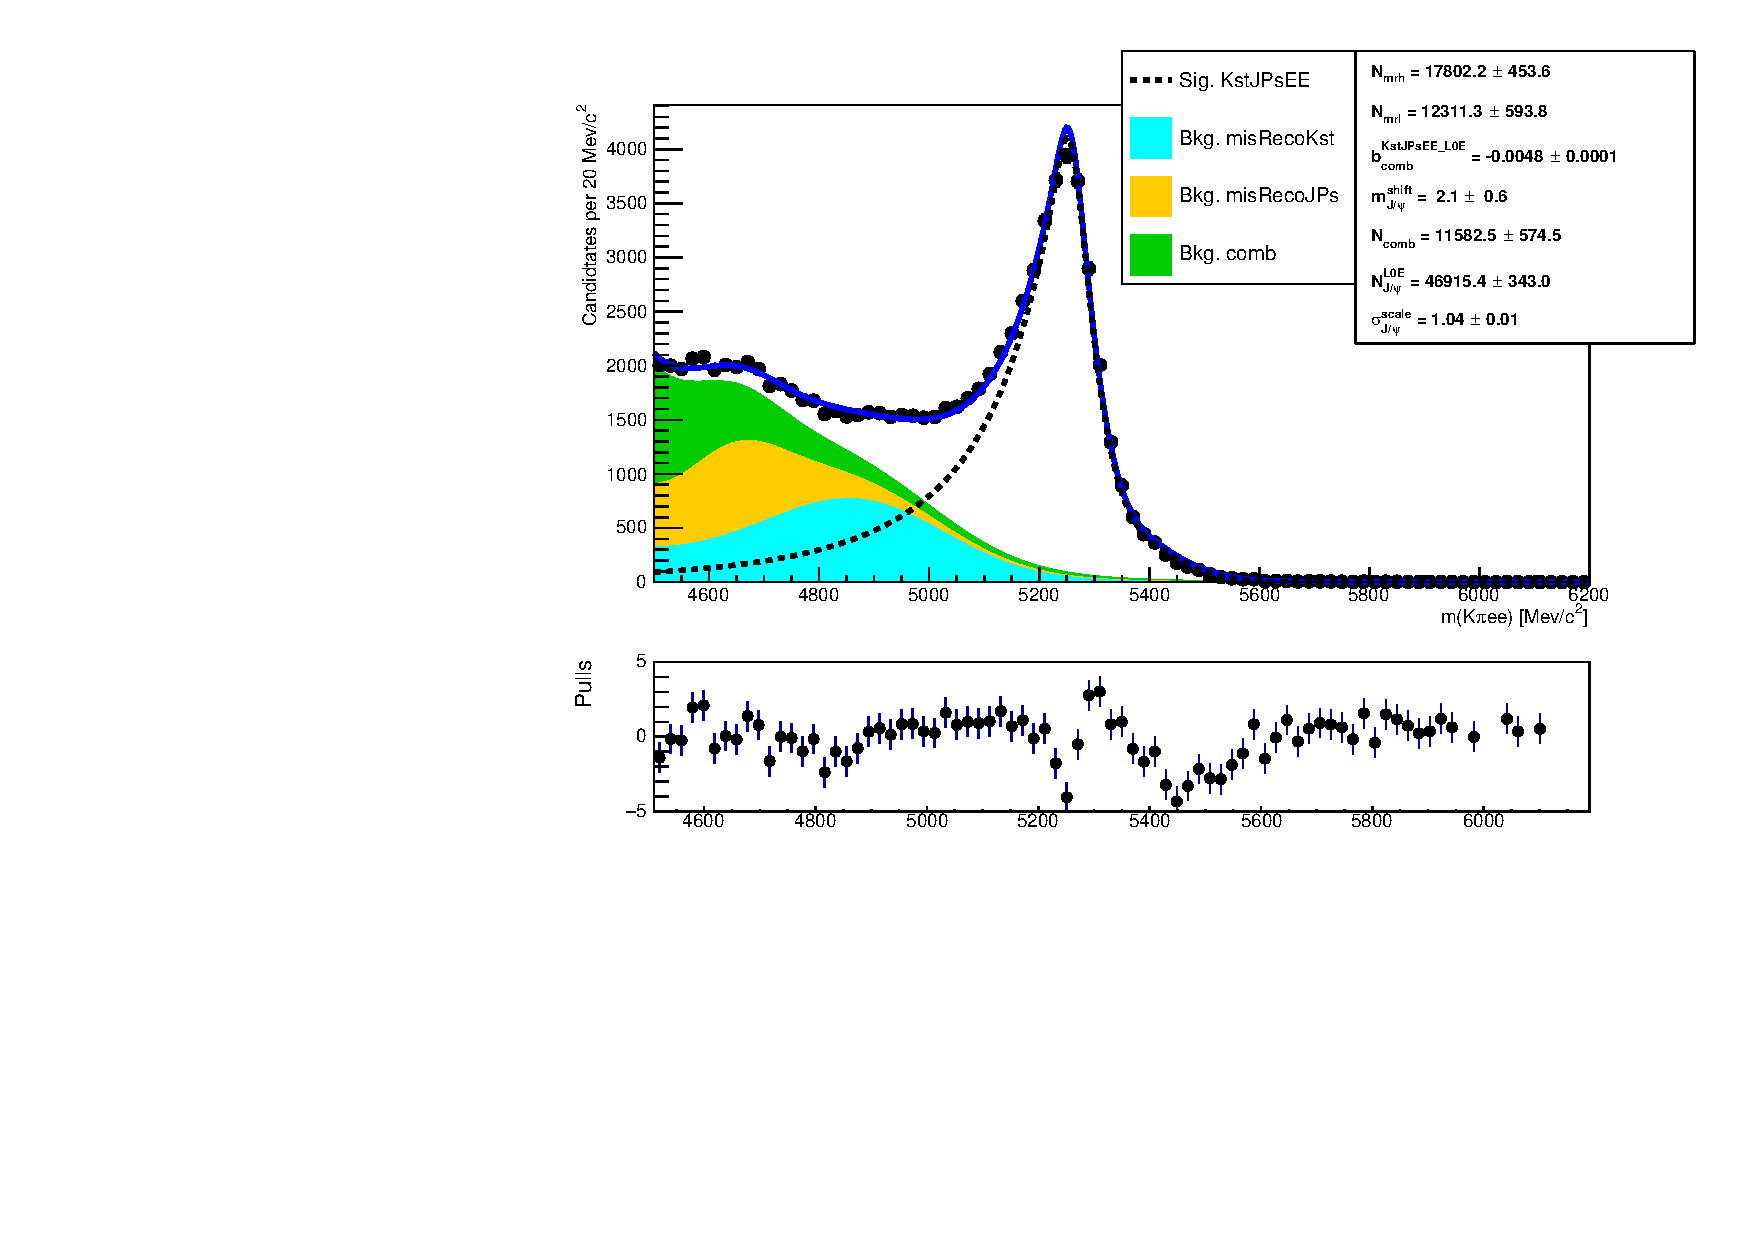
\includegraphics[width=0.46\textwidth]{RKst/figs/fit_EEs_0_EE-q2central-gmc/KstJPsEE_L0E_fitAndRes.pdf}
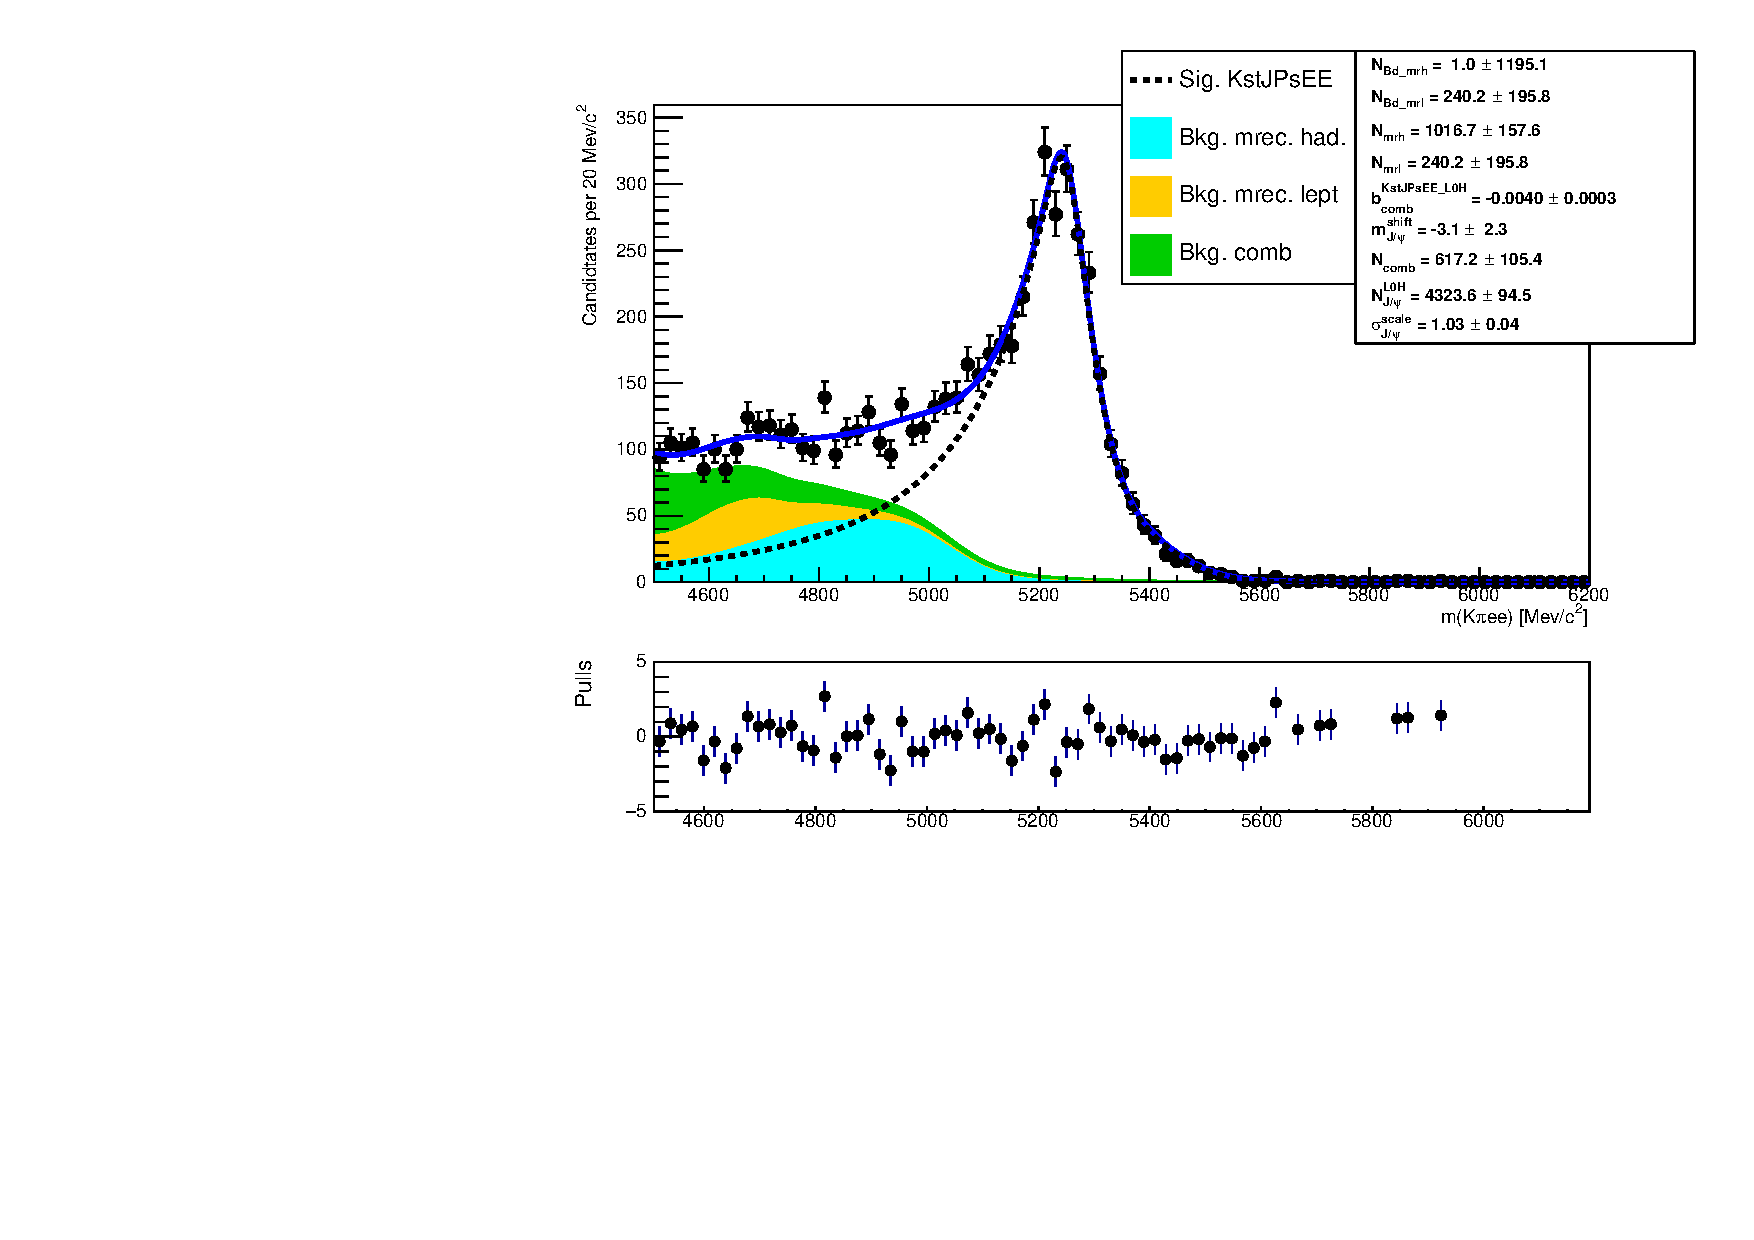
\includegraphics[width=0.46\textwidth]{RKst/figs/fit_EEs_0_EE-q2central-gmc/KstJPsEE_L0H_fitAndRes.pdf}
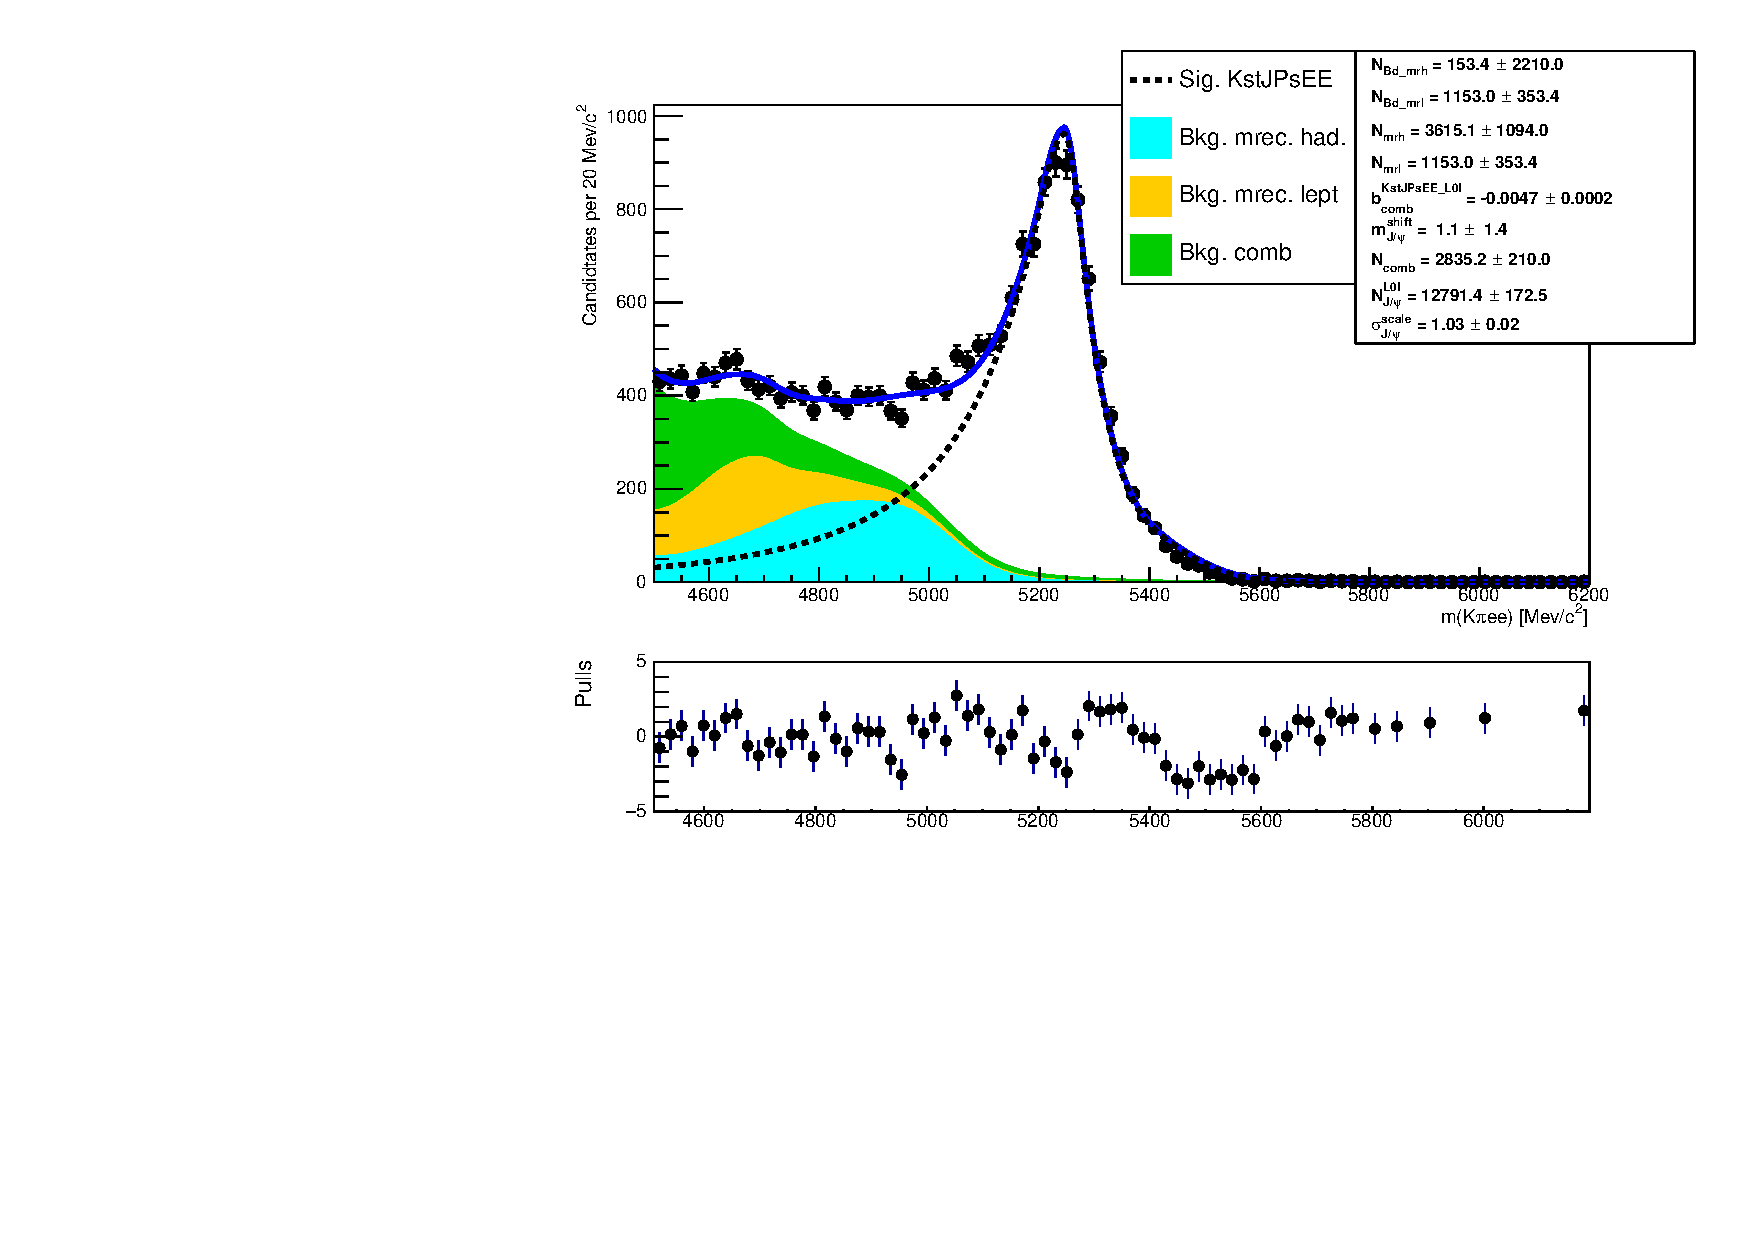
\includegraphics[width=0.46\textwidth]{RKst/figs/fit_EEs_0_EE-q2central-gmc/KstJPsEE_L0I_fitAndRes.pdf}
\caption{Fitted $m(K\pi ee)$ mass spectrum of $B^0 \rightarrow K^{*0} J/\psi(J/\psi\rightarrow ee)$
real data events in the three trigger categories. }
\label{fig:FitJpsiEE_Data_inTrigCat}
\end{figure}
%
\begin{figure}[h!]
\centering
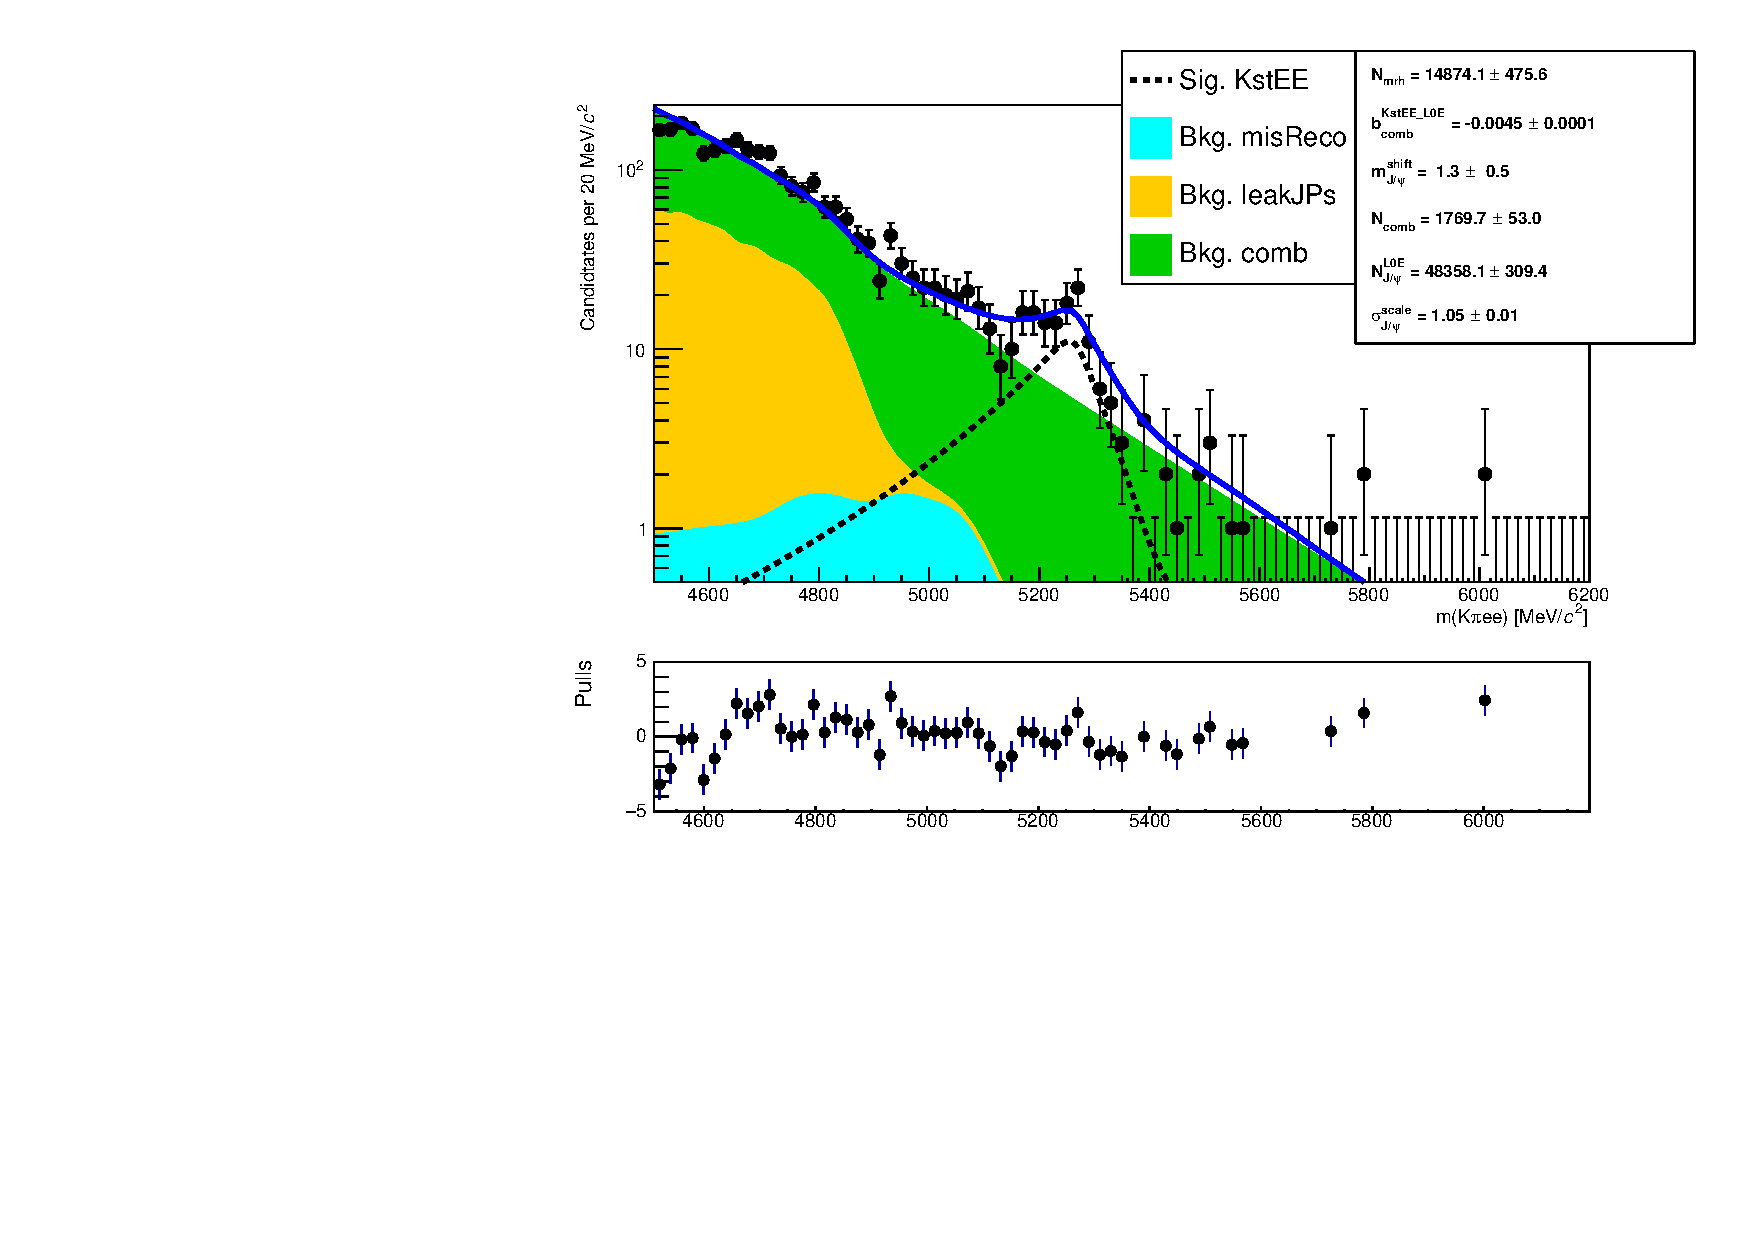
\includegraphics[width=0.46\textwidth]{RKst/figs/fit_EEs_0_EE-q2central-gmc/KstEE_L0E_log_fitAndRes.pdf}
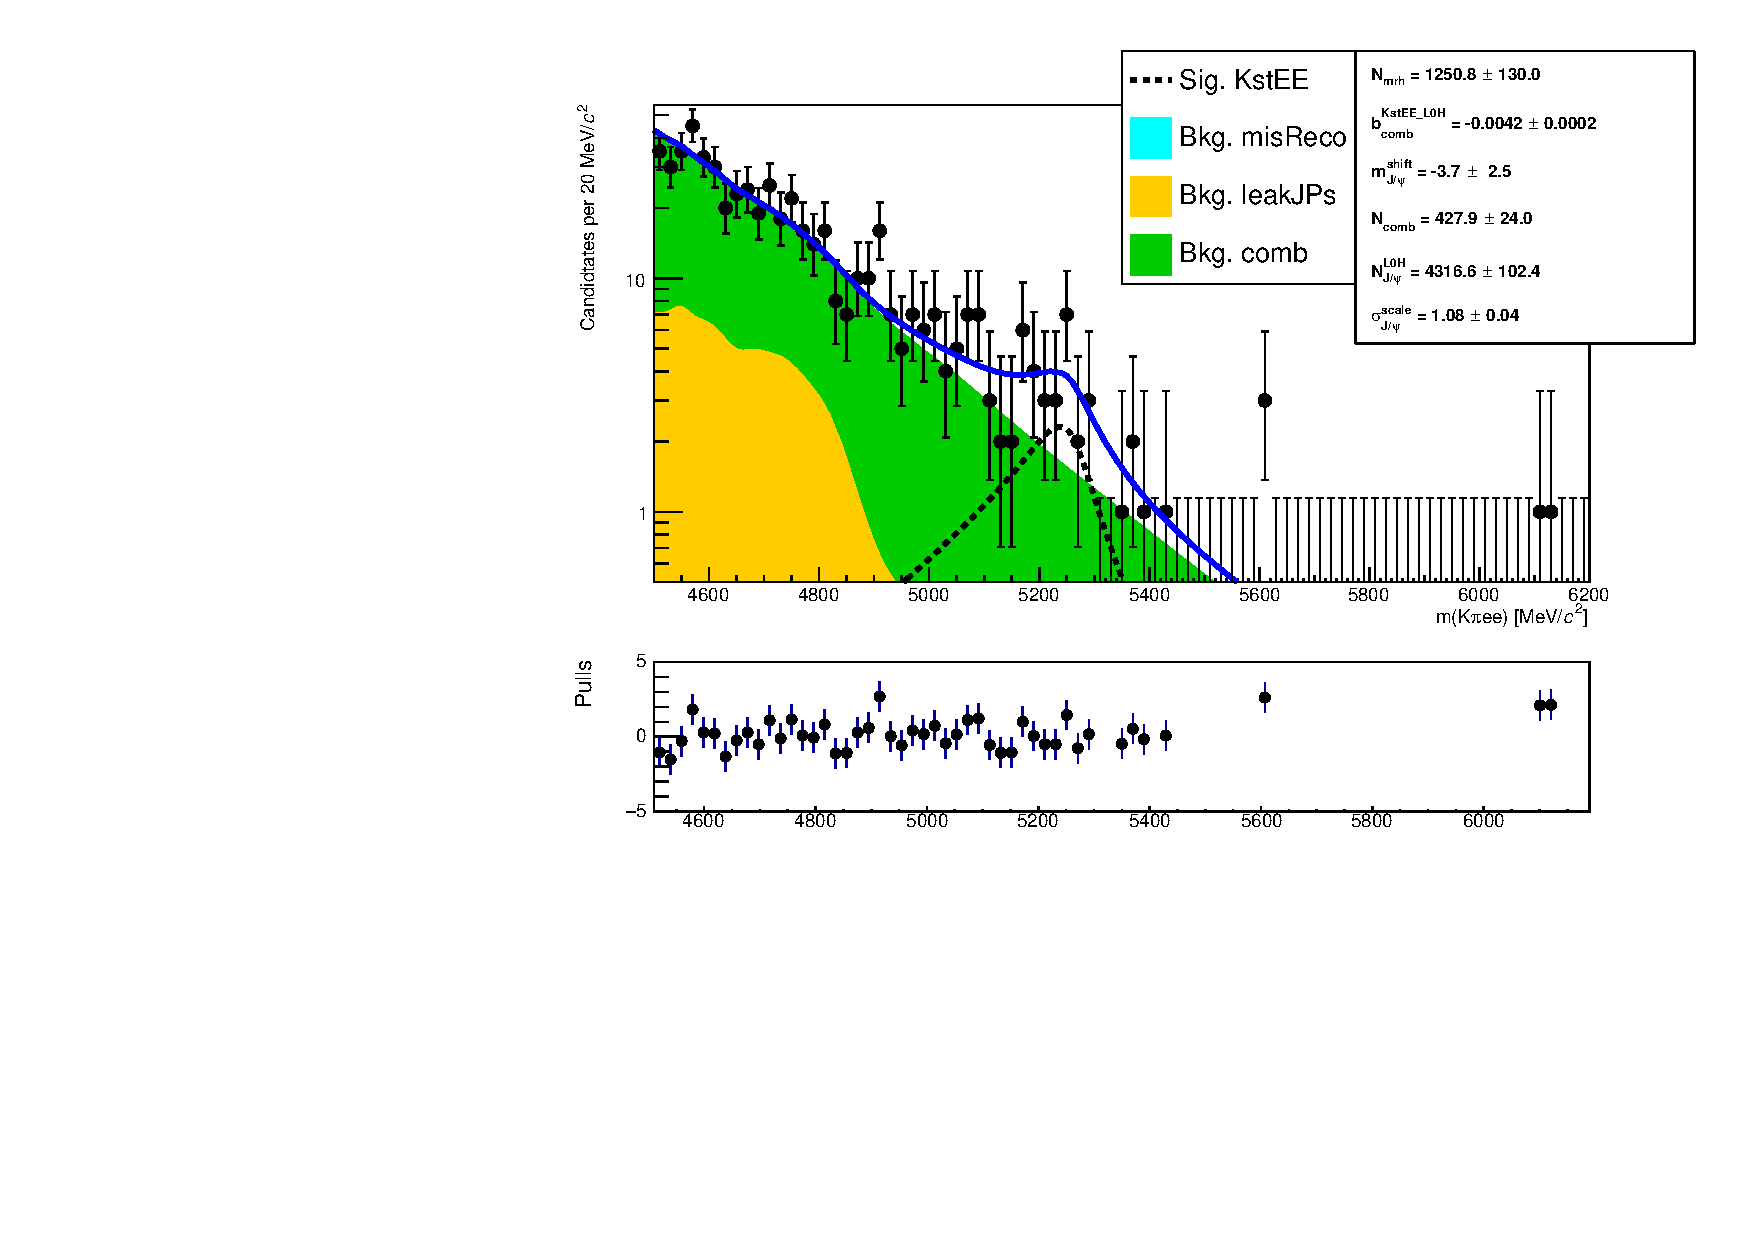
\includegraphics[width=0.46\textwidth]{RKst/figs/fit_EEs_0_EE-q2central-gmc/KstEE_L0H_log_fitAndRes.pdf}
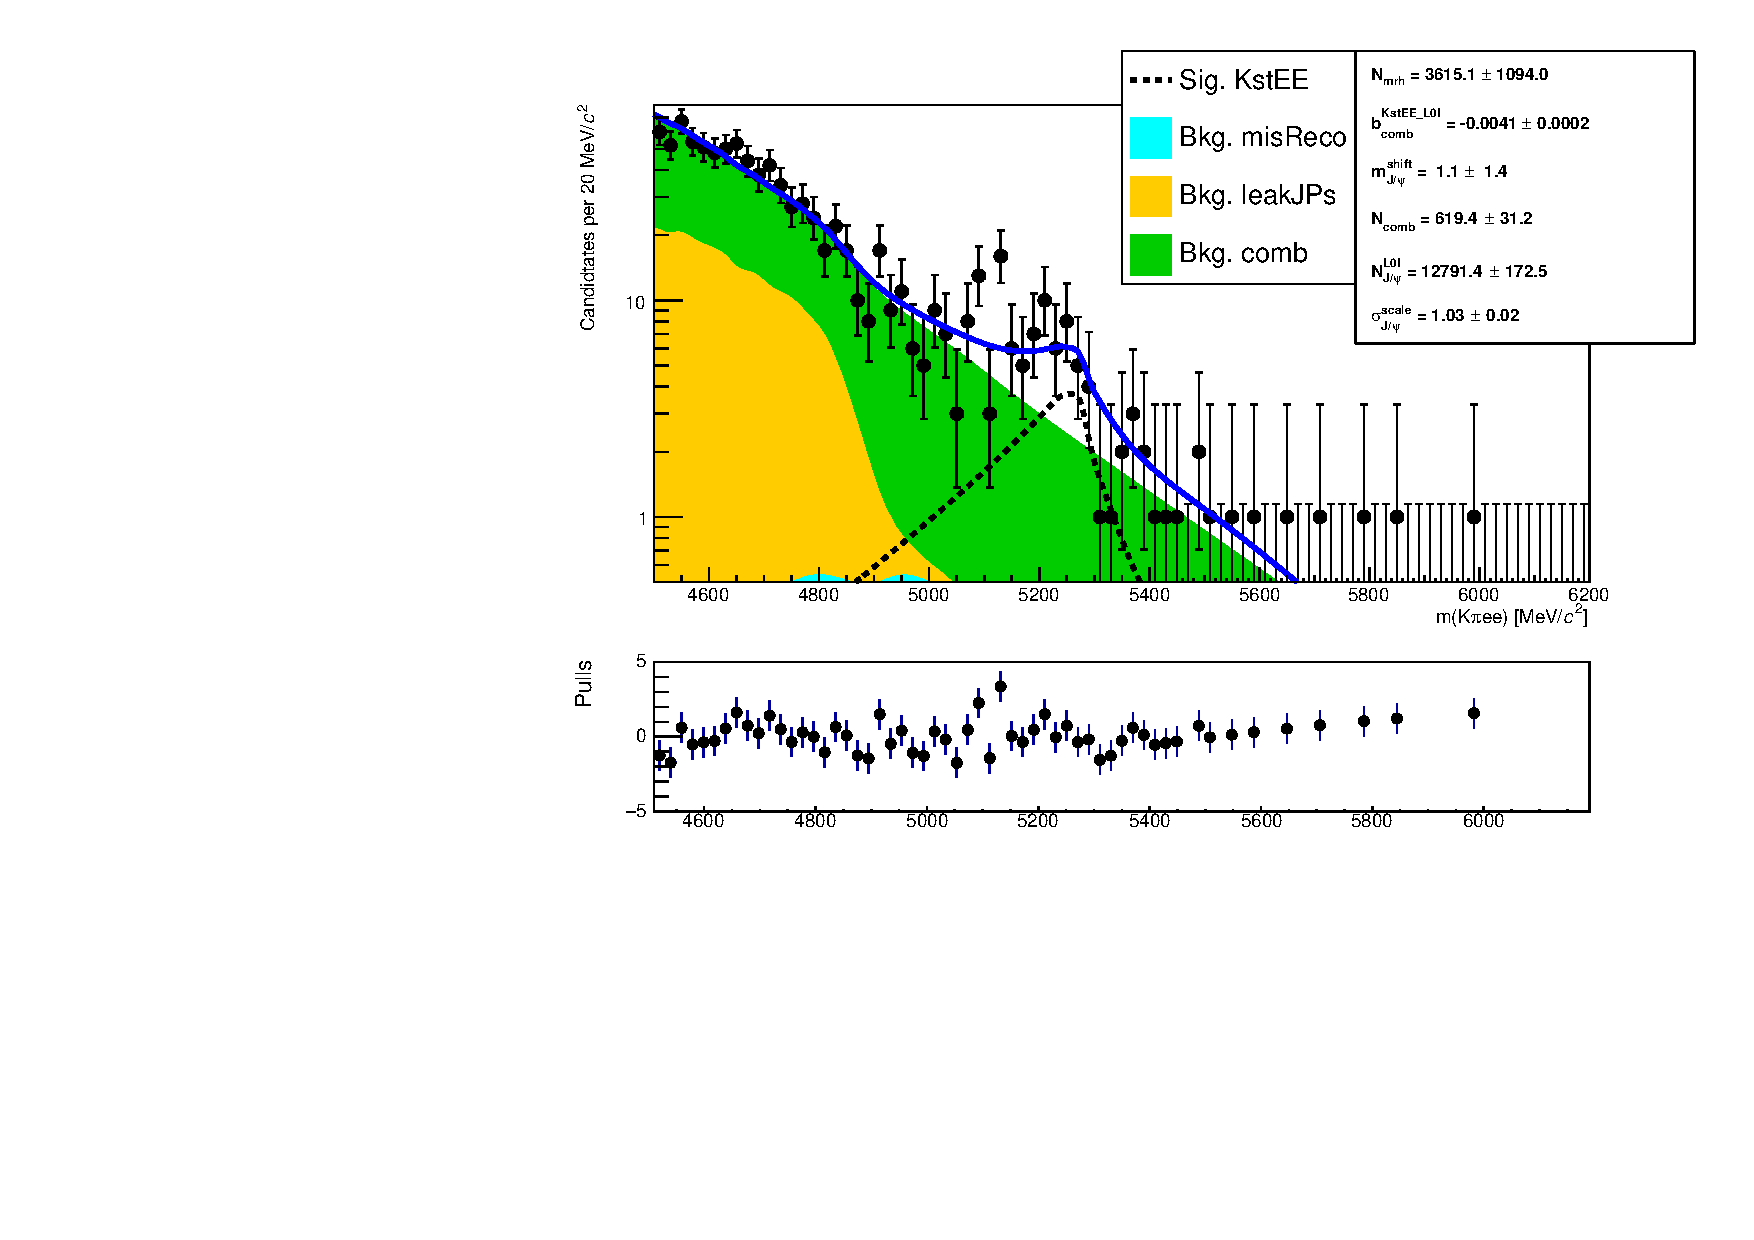
\includegraphics[width=0.46\textwidth]{RKst/figs/fit_EEs_0_EE-q2central-gmc/KstEE_L0I_log_fitAndRes.pdf}
\caption{Fitted $m(K\pi ee)$ mass spectrum of \BdKstee real data events in the three trigger categories and no photon emitted. }
\label{fig:FitEE_Data_inTrigCat}
\end{figure}


\subsection{Electron channels fits in the high \qsq interval}

In the high \qsq interval, above 15 \gevgevcccc, the efficiency for the
L0Hadron trigger becomes very low as the \Kstar has very low momentum.
In this region only 9 candidates are found spread in the interval
$4500 < m(K\pi ee) < 6000$ \mevcc. In the L0TIS category,
even if the yield is bigger a clear peak cannot be seen, therefore
only L0Electron triggered events are used in this region.

The signal PDF is described in the same way as for the central bin.
Simulated events are divided in three bremsstrahlung categories and fitted
using the same PDFs described in Sec.~\ref{sec:fit_ee_central}.
While the signal tail parameters are similar for the \jpsi and central \qsq samples
in the case of the high \qsq interval it is particularly important to keep them independent.
In fact, as can be seen in Fig.~\ref{fig:high_central_mass_comparison}, the invariant mass
distributions are significantly different for the two intervals.
The fractions of 0, 1 and 2 $\gamma$ components used to build the total PDF
are also in this case taken from simulated events are are reported in Tab.~\ref{tab:brem_frac_highq2}.

\begin{table}
\centering
\begin{tabular}{l|ccc}
Sample 	&	$0 \gamma$	&	$1 \gamma$  &	 $2 \gamma$  \\ \hline
\psitwos (L0E)			&	25.7 \%		&	52.1 \%		&	22.2 \%	 \\ \hline
15--20 \gevgevcccc (L0E)			&	20.7 \%		&	51.7 \%		&	27.6 \%	 \\ \hline
\end{tabular}
\caption{Percentages of events with 0, 1 and 2 emitted photons in the three
trigger categories, extracted from simulated events.}
\label{tab:brem_frac_highq2}
\end{table}

The background components, as for the central \qsq interval, include a combinatorial background
and a misreconstructed background coming from the hadronic system. Furthermore there is a leakage
due to the \psitwos resonance, that is wide enough to contribute in \qsq above 15 \gevgevcccc.
The combinatorial background is modelled with {\em comb model for high q2}.

The misreconstructed component is modelled in the same way described for the central \qsq interval.
However, in this case, its yield is not linked to the resonant fit as it is not guaranteed
that the same fraction of misreconstructed background will be present in the \jpsi
and high \qsq intervals. On the other hand the misreconstructed background shape is better
defined at high \qsq and therefore its yield can be left floating in the fit.

The \psitwos leakage component is modelled from $\decay{\Bz}{\Kstar(\psitwos\to\ee)}$
simulated events with the same method used for the \jpsi leakage in the central \qsq interval.
The yield of this component is fixed to the yield of \psitwos as
\begin{equation}
N_{\ell\ell}^{leak} = N_{\psitwos} \cdot k^{MC} = N_{\psitwos} \cdot \frac{N_{leak}^{MC}}{N_{\psitwos}^{MC}}.
\end{equation}
 In order to do this the \psitwos yield, $N_{\psitwos}$, is obtained from a fit to the \psitwos invariant
 mass peak. Since we are only interested in the \psitwos yield we fit the $m(K\pi ee)$ obtained from
 a kinematic fit where the dimuon mass is constrained to the known \psitwos mass.
 This allows to eliminate the misreconstructed background form the fit mass window and
 use a simple model composed by a signal component and a combinatorial background component.
 The signal is described with a Double Crystal Ball function with opposite tails
 already described the \Lb fits (see Sec.~\ref{sec:Lb_fit}), and the combinatorial
 background is described with an exponential.
 The fit to the \psitwos peak is reported in Fig.~\ref{fig:fit_ee_highq2}
 together with the fit to the $\decay{\Bz}{\Kstar \ee}$ candidates in the high \qsq interval.
 
 \begin{figure}[h!]
\centering
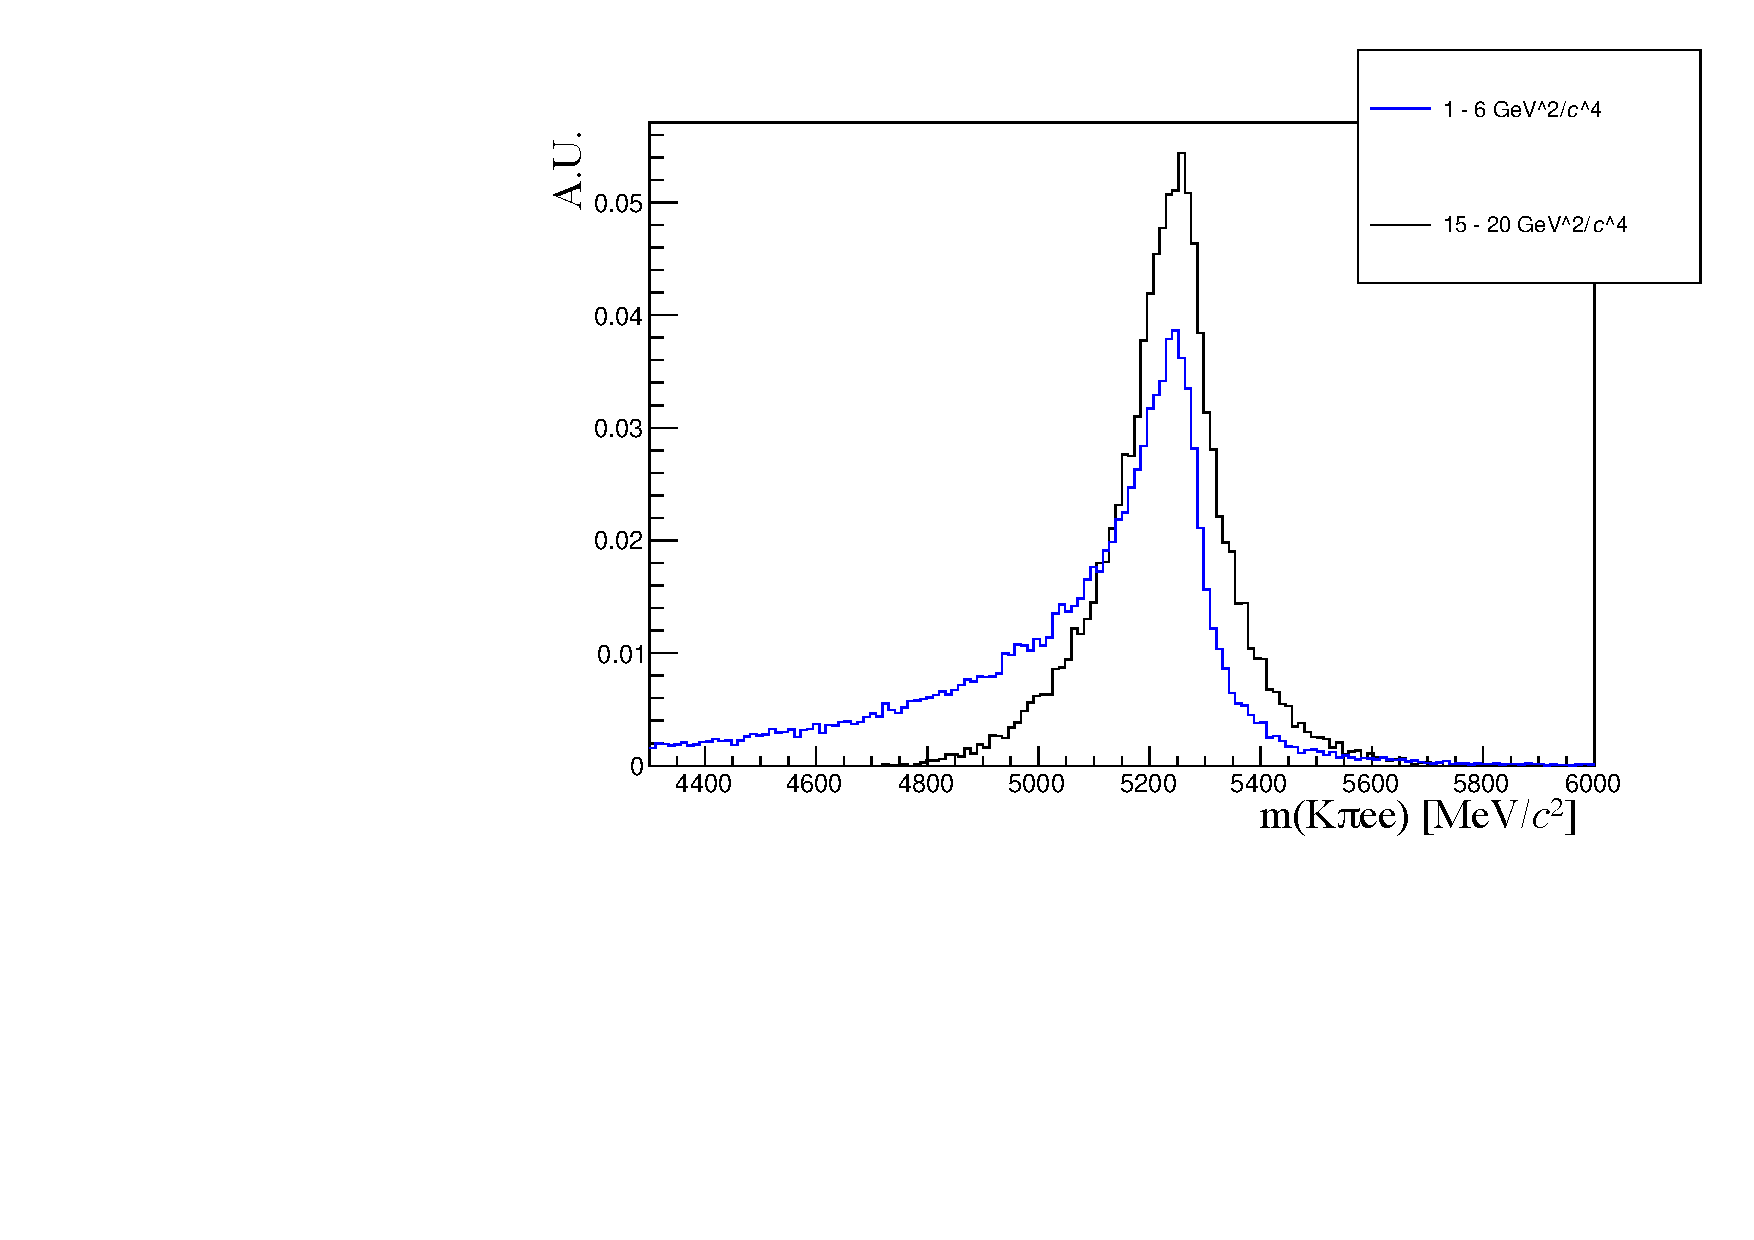
\includegraphics[width=0.70\textwidth]{RKst/figs/high_central_mass_comparison.pdf}
\caption{Simulated invariant mass of the $K\pi ee$ system in the $1 < \qsq < 6$ and $15 < \qsq < 20$ \gevgevcccc intervals.  }
\label{fig:high_central_mass_comparison}
\end{figure}

\begin{figure}[h!]
\centering
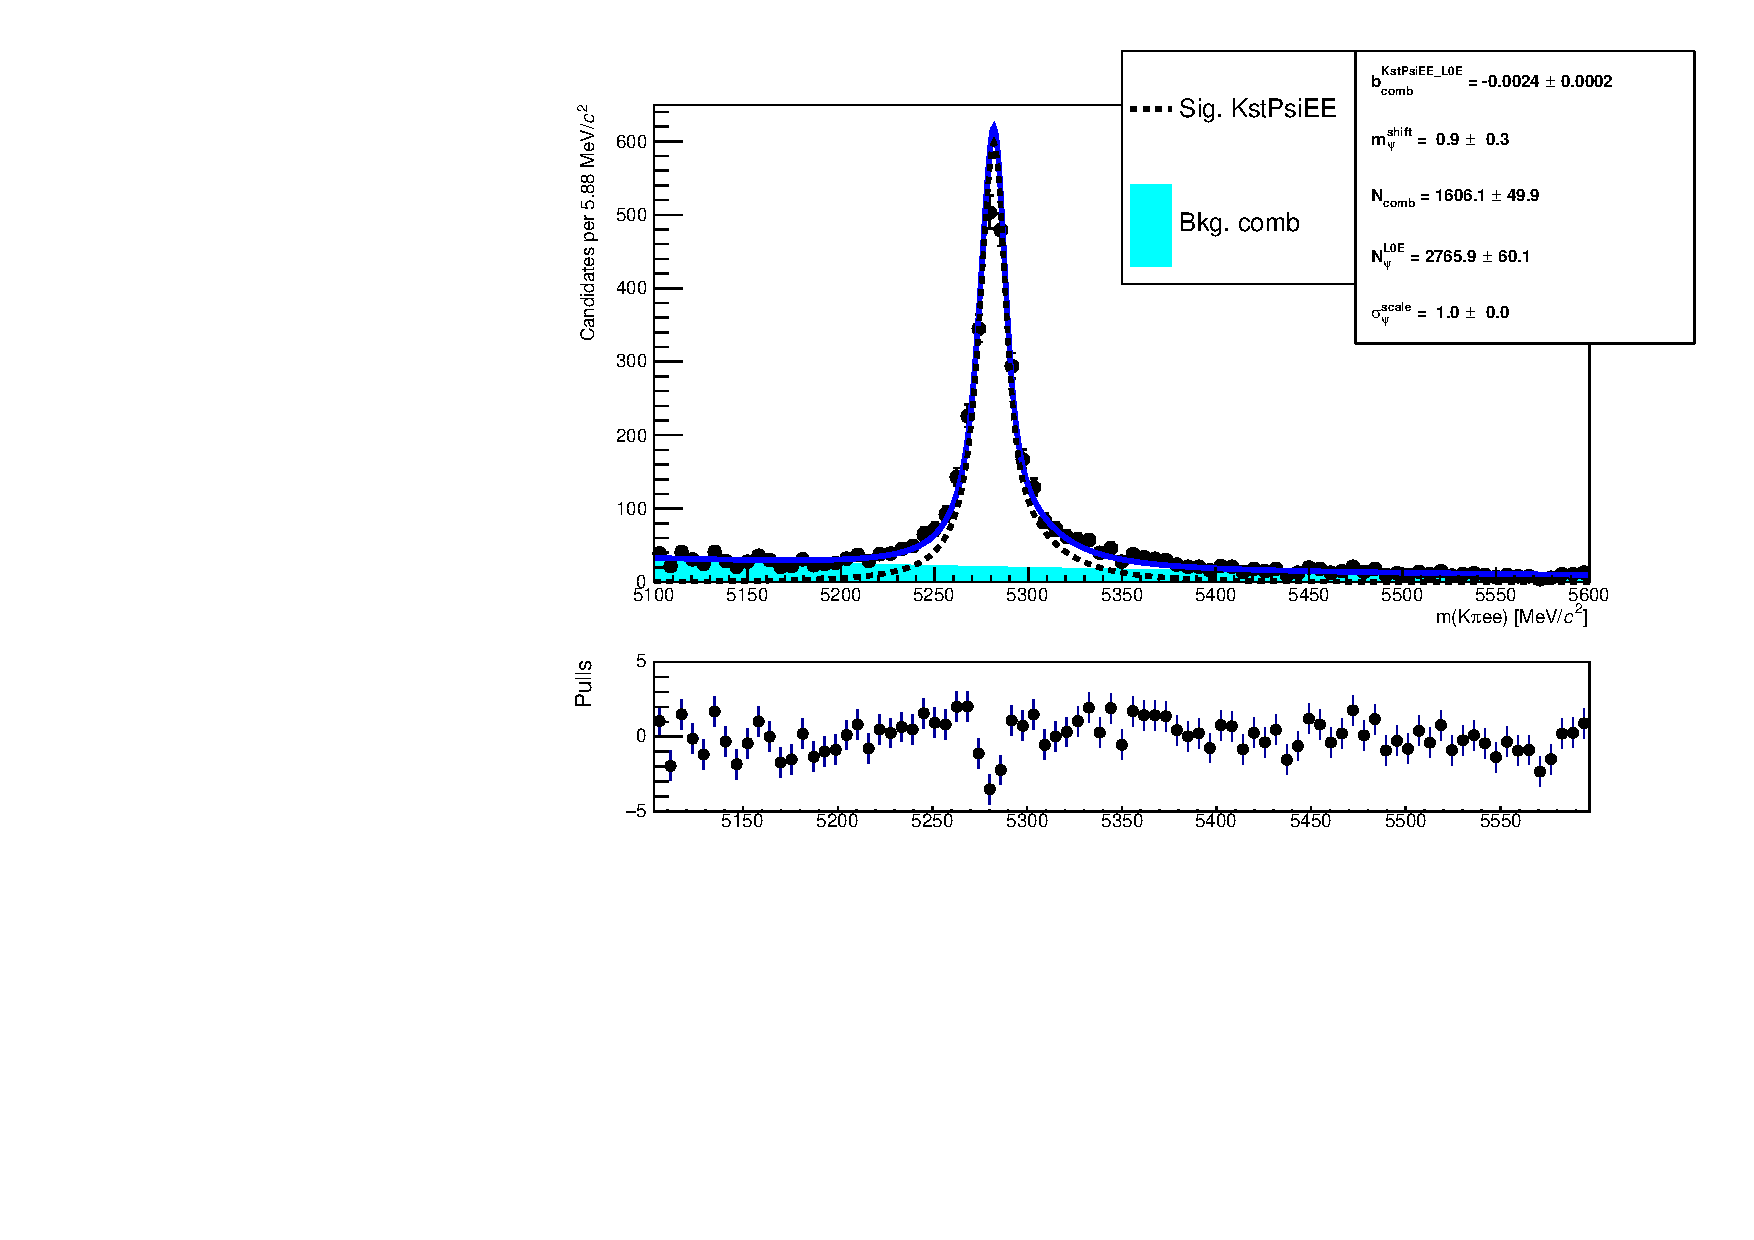
\includegraphics[width=0.48\textwidth]{RKst/figs/fit_EEs_0_EE-q2high-gmc/KstPsiEE_L0E_fitAndRes.pdf}
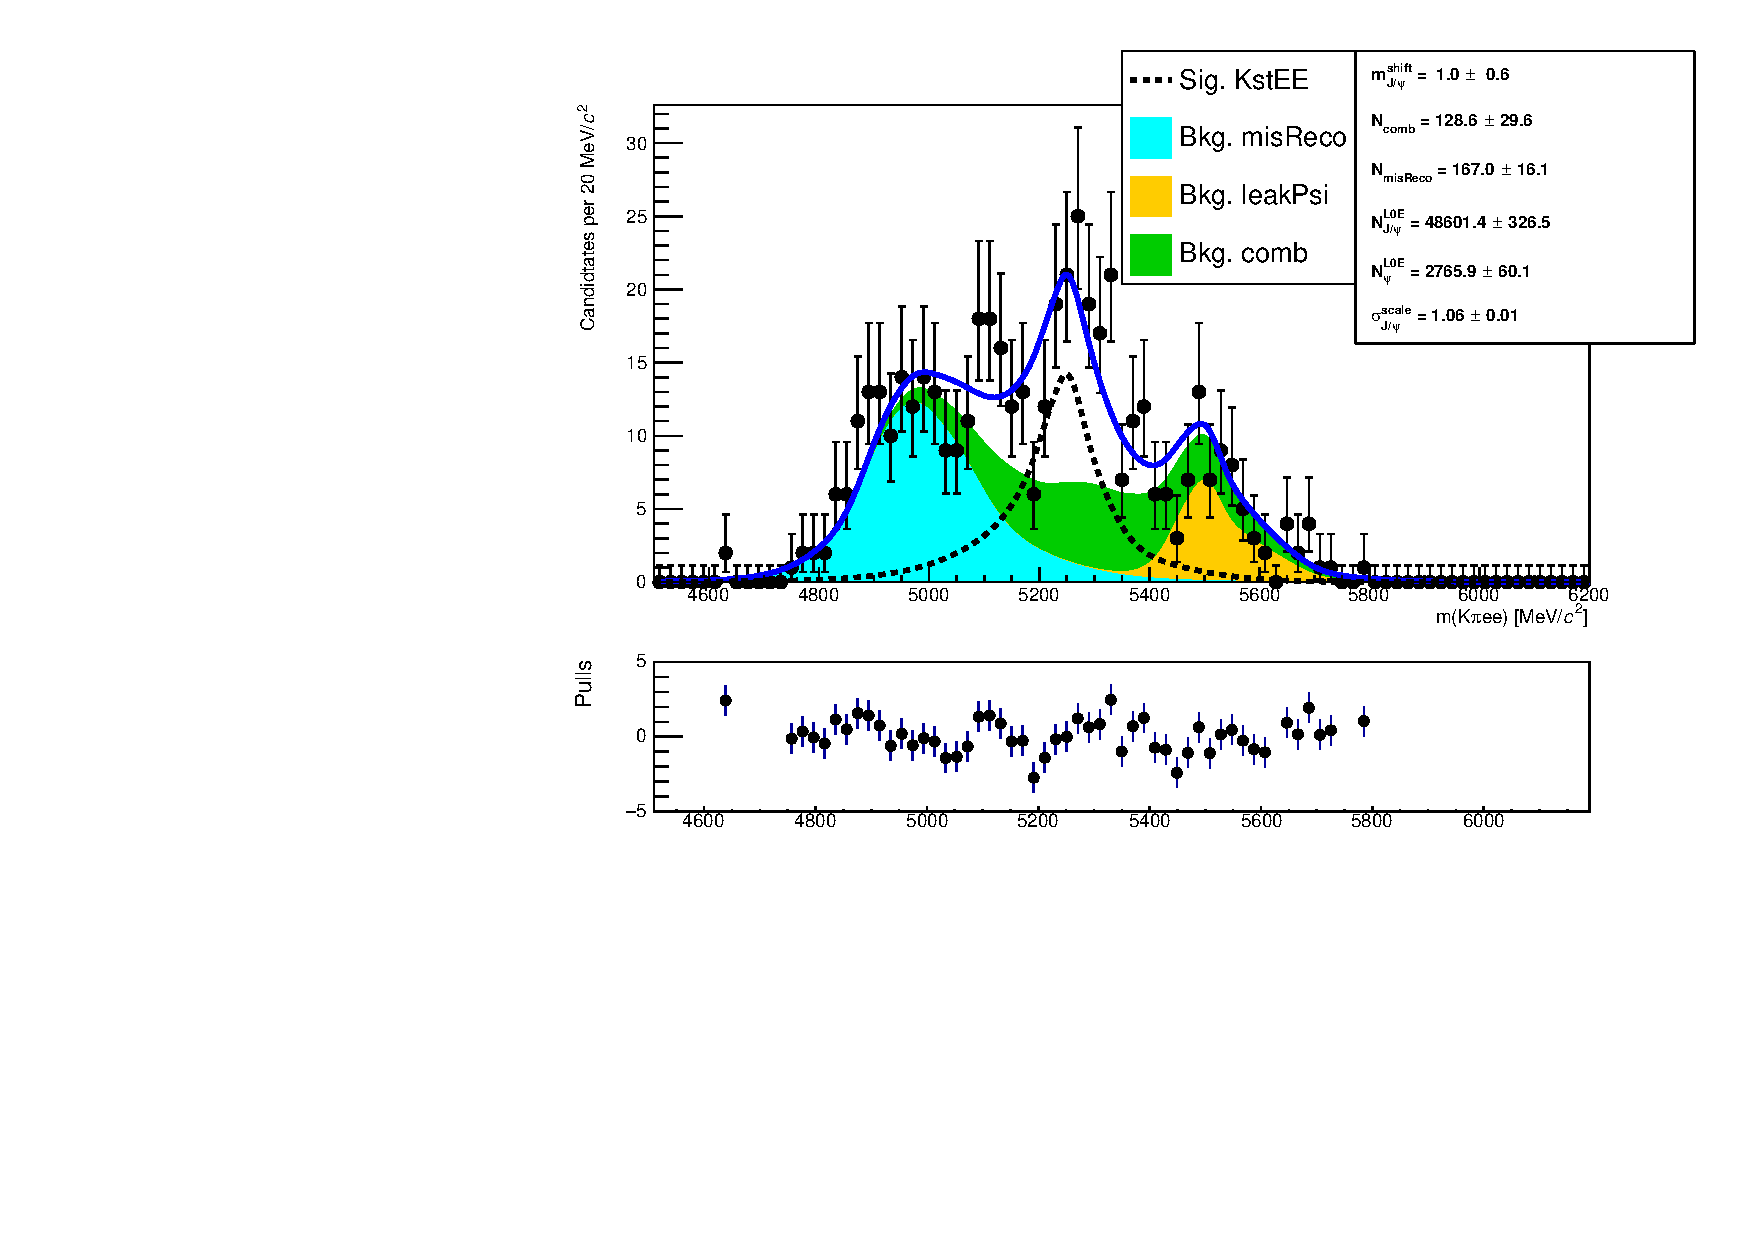
\includegraphics[width=0.48\textwidth]{RKst/figs/fit_EEs_0_EE-q2high-gmc/KstEE_L0E_fitAndRes.pdf}
\caption{Fitted $m(K\pi ee)$ invariant mass distribution in the \psitwos interval, $12 < \qsq < 25$ \gevgevcccc
and in the high \qsq interval, $15 < \qsq < 20$ \gevgevcccc }
\label{fig:fit_ee_highq2}
\end{figure}

\section{Fit summary}

In Tab.~\ref{tab:RKst_yields} are reported raw yields obtained from the
fits described in the previous sections. The values for the rare channels are not
directly floating in the fits but as described in Sec.~\ref{sec:rkst_fits} they are parameterised
as a function of the number of resonant events found and the ratios $R_{ee}$ and $R_{\mu\mu}$
between the resonant and rare branching fractions. Measured values of these ratios are reported 
in Tab.~\ref{tab:RKst_results}.

\begin{table}
\centering
\begin{tabular}{|c|c|c|c|}
\hline
 Sample 			& 1--6 GeV$^2/c^4$ 				& 15--20$ GeV^2/c^4$ 				& $J/\psi$  \\ \hline
$\mu\mu$ 			& $ 625.38  \pm  29.60 $ & $ 606.87  \pm  27.56 $ & $ 333917.20  \pm  599.73 $ \\
$ee$ L0Electron 	& $ 131.77  \pm  18.06 $ & $ 132.28  \pm  27.92 $ & $ 48103.10  \pm  329.77 $ \\
$ee$ L0Hadron 	& $ 32.50  \pm  4.50 $ & -- & $ 4439.51  \pm  98.38 $ \\
$ee$ L0TIS 	& $ 48.53  \pm  6.68 $ & -- & $ 12683.18  \pm  174.25 $ \\
\hline 
 \end{tabular}
\caption{Raw yields of events found fitting invariant mass distributions of the rare and resonant events. }
\label{tab:RKst_yields}
\end{table}


\clearpage

